\chapter{Descripción de los problemas en fluidos con transferencia de calor }
\graphicspath{{figs/cap4/}}
\label{cap4}

En el presente capíulo se realiza la descripción de los problemas con transferencia de calor para fluidos multifásicos con cambio de fase llevados a cabo para validar los códigos numéricos desarrollados, siendo éstos la \textit{Construcción de Maxwell}, la \textit{Estratificación de un fluido Van der Waals con temperatura no uniforme} y la \textit{Generación de burbujas en una superficie horizontal calefaccionada}.

\section{Construcción de Maxwell}

En esta sección se explica el procedimiento por el que a partir de una EOS, se puede obtener las densidades de coexistencia de un fluido para un dado valor de presión y temperatura. Dicho procedimiento se llama Construcción de Maxwell, donde necesariamente la EOS con la que se modela el fluido debe permitir la coexistencia de densidades para sus variables de estado. Para la resolución de éste problema solo se utiliza la ecuación hidrodinámica del LBM.

En el desarrollo del Cap. (\ref{cap2}) se adoptó como EOS del presente trabajo, la ecuación de VdW Ec. (\ref{eq:p_eos_4}) que describe el comportamiento de un gas real y permite la coexistencia de diferente densidad.

\begin{align}
	p = \frac{R T}{V_m - B} - A {\left(\frac{1}{V_m}\right)}^2
	\label{eq:p_eos_4}
\end{align}

La Ec. (\ref{eq:p_eos_4}) puede ser representada gráficamente en un diagrama $P - V_m$. A modo de ejemplo se presenta él diagrama para el caso del dióxido de carbono ($CO_2$) de tres temperaturas distintas en la Figura (\ref{fig:P_V_CO2}).  La temperatura de interés es la de $T = 270 \> K$, donde se vislumbra que en $p = 44,08 \> atm$ la gráfica se intersecta en tres valores de $V_m$, siendo dos de ellos estables; por lo que se observa que hay dos volúmenes molares de coexistencia, indicando las fases líquido y gaseosa \cite{huang2015multiphase}. 

\begin{figure}[htbp]
	\centering
	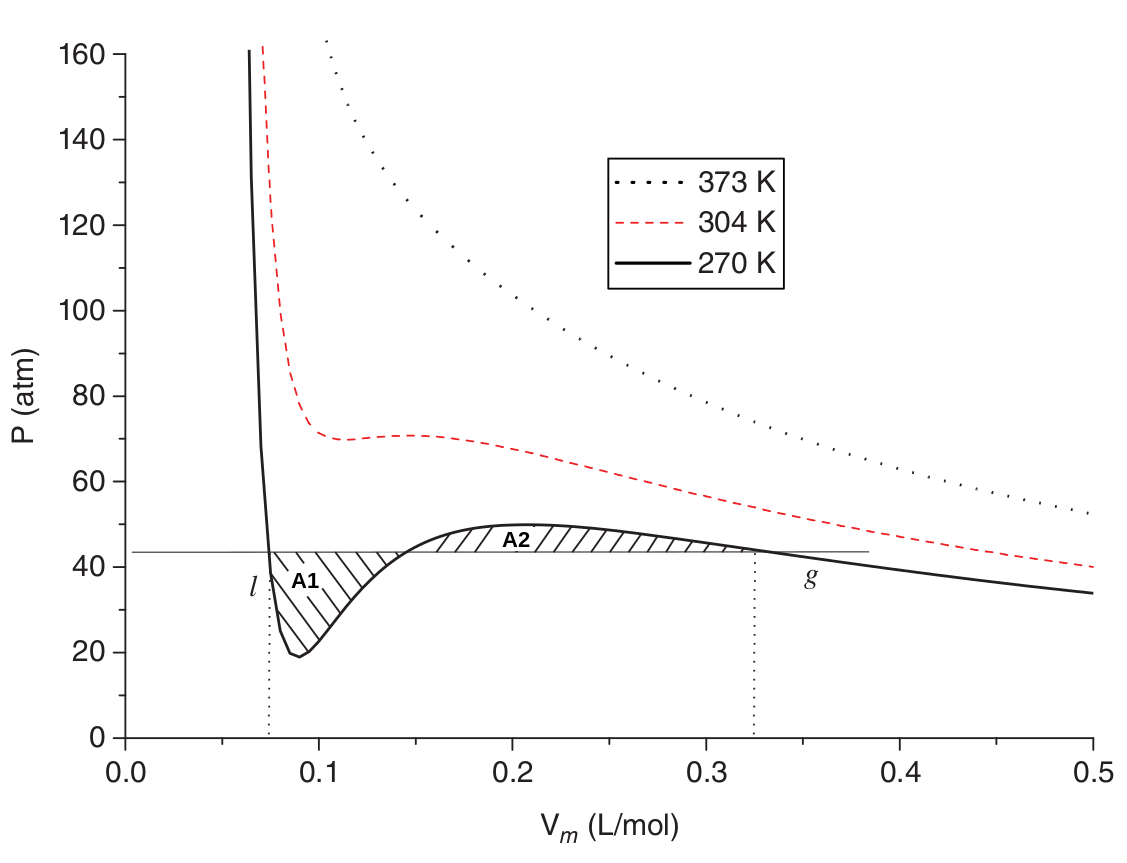
\includegraphics[width=.8\textwidth]{figs/cap4/Diagrama_P_V_del_CO2_Multiphase_LBM}
	\caption{Diagrama $P - V_m$ de la EOS de VdW del $CO_2$ con las constantes $a = 3,592$ y $b = 0,04267$, representando par a $T = 270 \> K$ los volúmenes molares del líquido y gas. \cite{huang2015multiphase}}
	\label{fig:P_V_CO2}	
\end{figure}

La construcción de Maxwell, también llamada regla de igualdad de áreas, indicada en Ec. (\ref{eq:maxwell_Construction}), es un procedimiento analítico para encontrar las densidades de coexistencia del líquido y gas. Donde $P$ es la presión de la EOS y $p_0$ es una presión constante. Al realizar la integral propuesta surge que las áreas \textbf{A1} y \textbf{A2} de la Figura (\ref{fig:P_V_CO2}) deben ser iguales.

\begin{equation}
\int_{V_{m,l}}^{V_{m,g}} P d V_m = p_0 (V_{m,l} -  V_{m,g})
\label{eq:maxwell_Construction}
\end{equation}

La Ec. (\ref{eq:p_eos_4}) se puede re-estructurar como Ec. (\ref{eq:p_VdW_rho}) puesto que $\rho = \frac{1}{v}$, siendo $v$ el volúmen másico y relacionando $V_m$ con $v$ según cada fluido. Donde para un dado valor de temperatura tendremos la coexistencia de fases con su densidad $\rho_l$ para la fase líquida y $\rho_g$ para la gaseosa.

\begin{equation}
	p_{EOS} = \frac{\rho R T}{1- \rho b} - a {\rho}^{2} 
	\label{eq:p_VdW_rho}
\end{equation}

Para un dado valor de temperatura, llamado temperatura crítica (\textit{$T_c$}) comienzan a coexistir las dos fases. En el ejemplo mostrado de la Figura (\ref{fig:P_V_CO2}) $T_c = 304 \> K$. Analíticamente $T_c$ surge de aplicar el criterio de la primera y segunda derivada a la Ec.(\ref{eq:rho}) como se indica en Ec.(\ref{eq:criterio_1_2_deriv}) y se deben conocer los parámetros \textit{a} y \textit{b}.

\begin{equation}
	\frac{\partial\> p}{\partial\> V_{m}} = 0 \qquad \qquad \frac{\partial^{2} \> p}{\partial\> {V_{m}}^{2}} = 0
	\label{eq:criterio_1_2_deriv}
\end{equation}

Realizando adecuadamente la adimensionalización  de la Ec.(\ref{eq:p_VdW_rho}) se puede graficar una curva de coexistencia $T_r - \rho_r$, donde $T_r = \frac{T}{T_c}$, $\rho_r = \frac{\rho}{\rho_c}$ y $T_c$ es calculado a partir de los parámetros \textit{a} y \textit{b} asignados al fluido de estudio. Es de importancia destacar que las curvas de coexistencia dependen de la EOS que se esté utilizando para describir el comportamiento del fluido. En el caso de estudio analizado, la EOS es de VdW y la curva de coexistencia es universal, independientemente de los parámetros \textit{a} y \textit{b}, debido a que se encuentra normalizada por unidades críticas.

En éste problema, se valida la curva de coexistencia $T_r - \rho_r$ calculada analíticamente para un fluido con una EOS de VdW, como la observada en la Figura (\ref{fig:v_760_MxC_c_simple}). 

Para un fluido con una EOS de VdW con su respectivos parámetros \textit{a} y \textit{b}, se puede calcular los valores de $T_c$ y $\rho_c$. Para  el fluido mencionadado en una cavidad bidimensional a una dada temperatura e inicializando la densidad del mismo aleatoriamente alrededor de  $\rho_c$, cuando se deje evolucionar en el tiempo se producirá la separación de las fases del mismo, produciéndose una coexistencia de fases. Por medio de la obtención de las densidades de coexistencia para distintas temperaturas iniciales, se puede reconstruir la curva de coexistencia analítica.

\subsection{Validación}

La validación de éste problema se hizo utilizando los parámetros $a =0,5$ y $b = 4,0$; para un tamaño de malla de 201 x 201 nodos y $T_r$ variando con un paso de $0,025$ en el rango de $[0,6 - 0,975]$.  El valor de los parámetros utilizados de LBM son los siguientes:

\begin{align*}
diag(\mathbf{\Lambda}) = 
\begin{bmatrix}
1.0 & 0.8 & 1.1 & 1.0 & 1.1 & 1.0 & 1.1 & 0.8 & 0.8 \\
\end{bmatrix}\\
G = -1.0 \quad c = 1.0 \quad \sigma = 0.125 \quad a = 0.5 \quad b = 4.0 \\
\mathbf{g} = (0.0 \quad 0.0 \quad 0.0 ) \qquad \rho_c = \frac{1}{12} \qquad T_c = 0.037037037
\end{align*}

La Figura(\ref{fig:v_760_MxC_c_simple}) muestra la validación del código realizado en \textsc{C} para simple precisión en una CPU Intel Core i7-3770; con distintos parámetros $\sigma$ del modelo MRT, donde se observa que el valor de $\sigma = 0,125$ es el que mejor ajusta a la curva de coexistencia como se discute en \cite{fogliatto2018modelado}. La Figura (\ref{fig:v_760_MxC_cuda_simple}) muestra el resultados obtenidos del código realizado en \textsc{Cuda C} en simple precisión en la misma GPU.

Los resultados de las Figuras (\ref{fig:v_760_MxC_c_simple}) y (\ref{fig:v_760_MxC_cuda_simple}) se realizaron en 50000 pasos de tiempo en cada uno de los valores de $T_r$. El valor obtenido de las densidades de coexistencia de fases entre los códigos de \textsc{C} y \textsc{Cuda C} resultan similares en primera instancia. 

El resultado que se obtuvo de realizar la validación en doble precisión es que los dos códigos desarrollados obtienen el mismo valor en las densidades de fase.

\begin{figure}[h!]
	\centering
	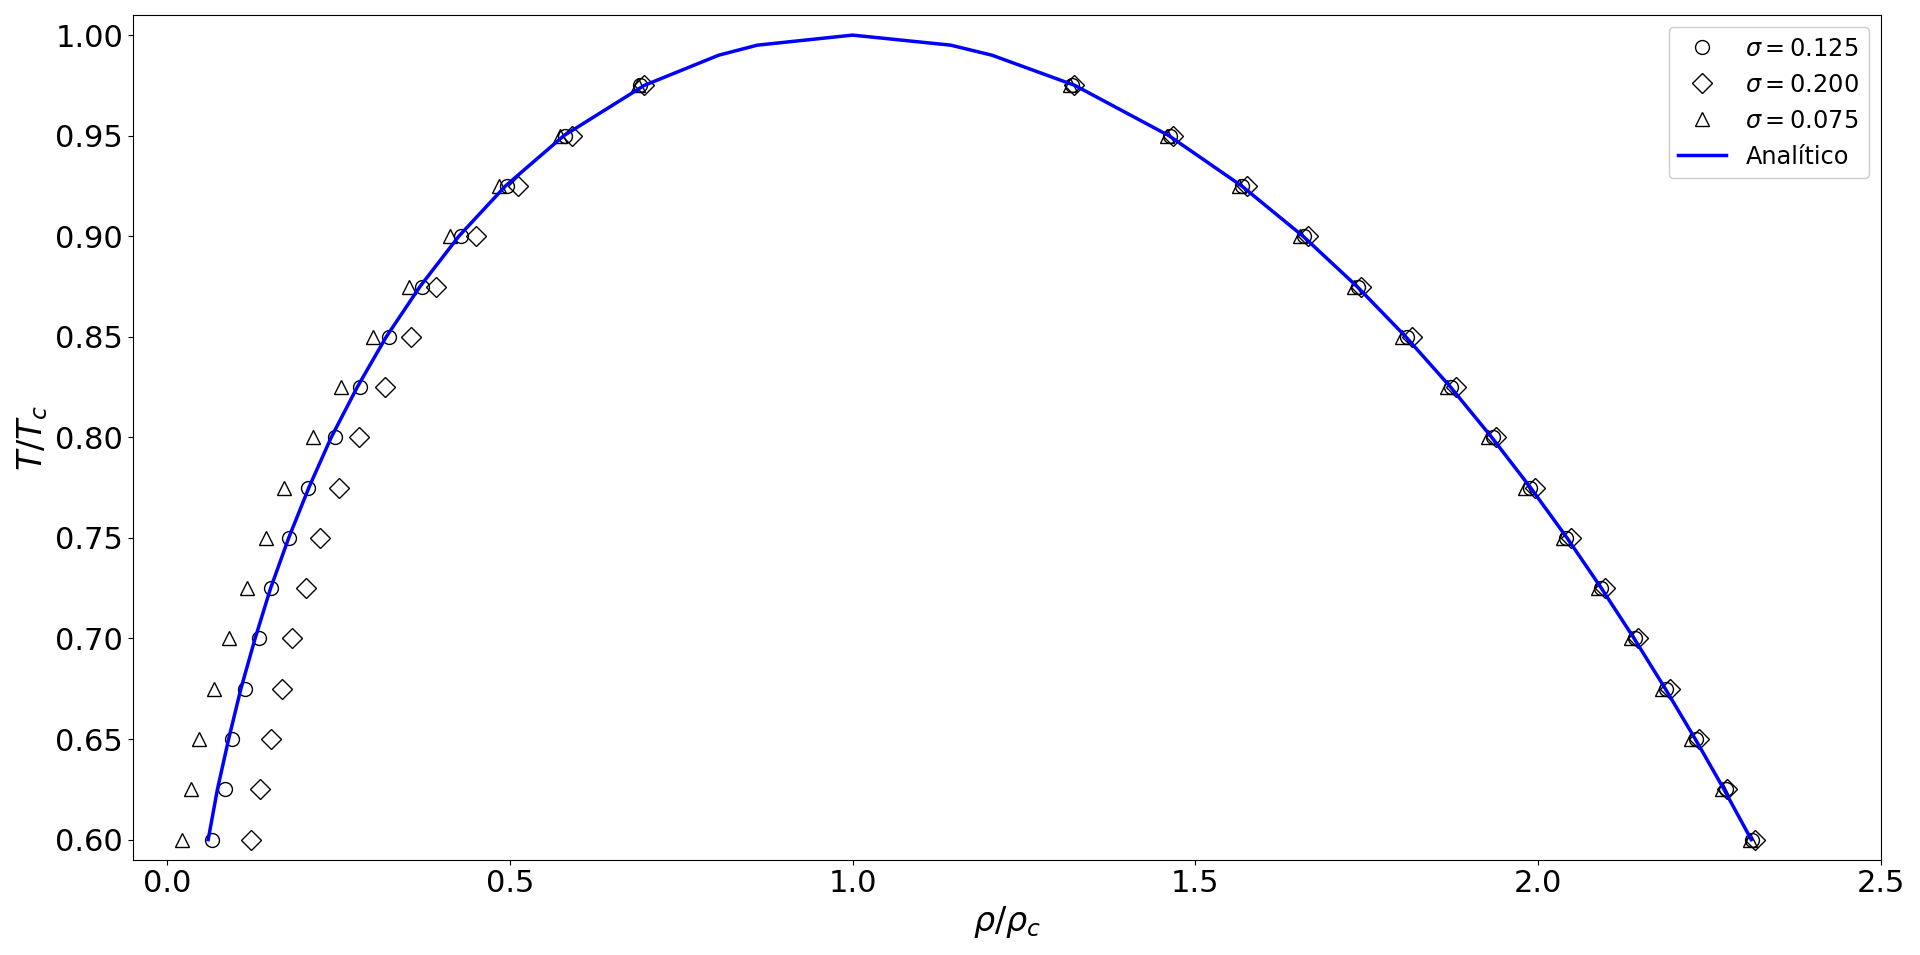
\includegraphics[width=\textwidth]{figs/cap4/v_760_MxC_c_simple}
	\caption{Curva de coexistencia de fases para un fluido de VdW con los parámetros $a = 0,5 $ y $b = 4,0 $, obtenida en simple precisión en la GPU NVIDIA GeForce GTX 760 en el código desarrollado en \textsc{C}. $\sigma = 0.075[\bigtriangleup]$	 $\sigma = 0.125[\bigcirc]$ y $\sigma = 0.200[\diamondsuit]$ }
 	\label{fig:v_760_MxC_c_simple}	
\end{figure}

\begin{figure}[h!]
	\centering
	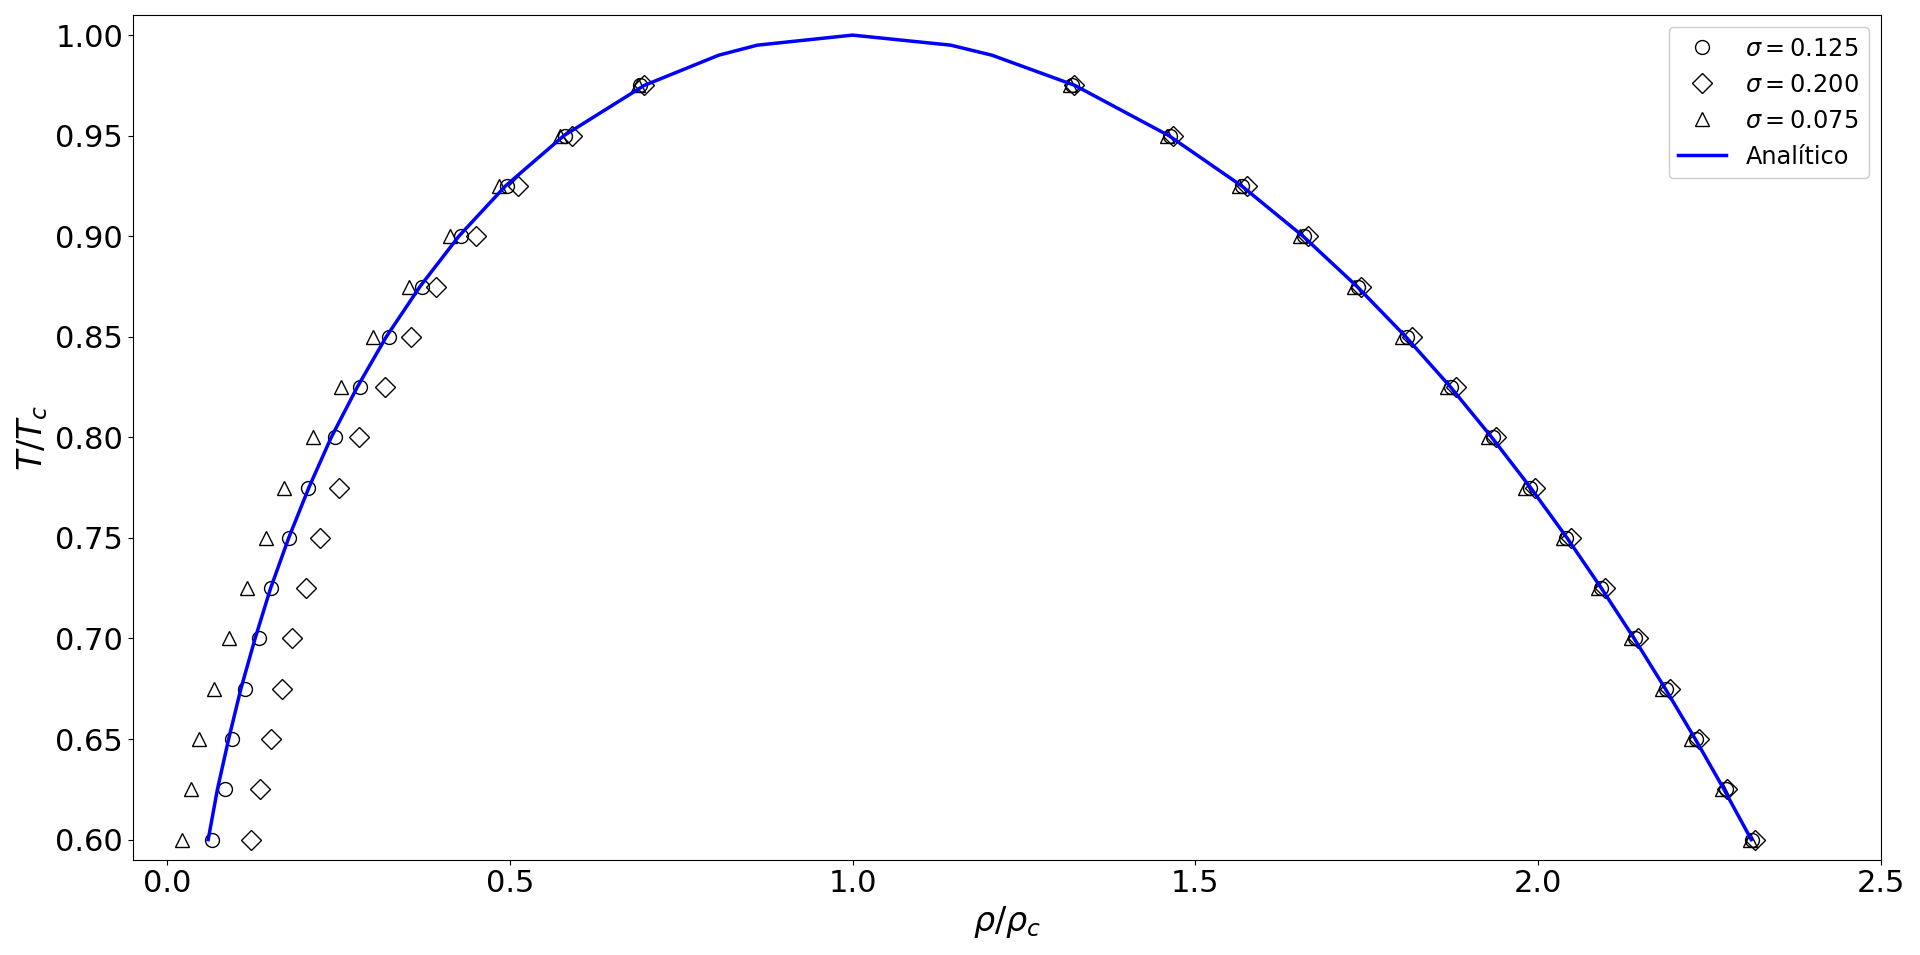
\includegraphics[width=\textwidth]{figs/cap4/v_760_MxC_cuda_simple}
	\caption{Curva de coexistencia de fases para un fluido de VdW con los parámetros $a = 0,5 $ y $b = 4,0 $, obtenida en simple precisión en la GPU NVIDIA GeForce GTX 760 en el código desarrollado en \textsc{Cuda C}. $\sigma = 0.075[\bigtriangleup]$	 $\sigma = 0.125[\bigcirc]$ y $\sigma = 0.200[\diamondsuit]$ }
	\label{fig:v_760_MxC_cuda_simple}	
\end{figure}



\newpage
\subsection{Comparación de precisiones}

En el análisis de la comparación de las precisiones, sólo se presentan los resultados obtenidos mediante el código de \textsc{C}, debido a que los resultados de \textsc{Cuda C} son idénticos.

La Figura (\ref{fig:v_760_MxC_c_comparacion}) muestra los resultados de las densidades de coexistencia de fases para simple y doble precisión, no siendo apreciable la diferencia.

\begin{figure}[htbp]
	\centering
	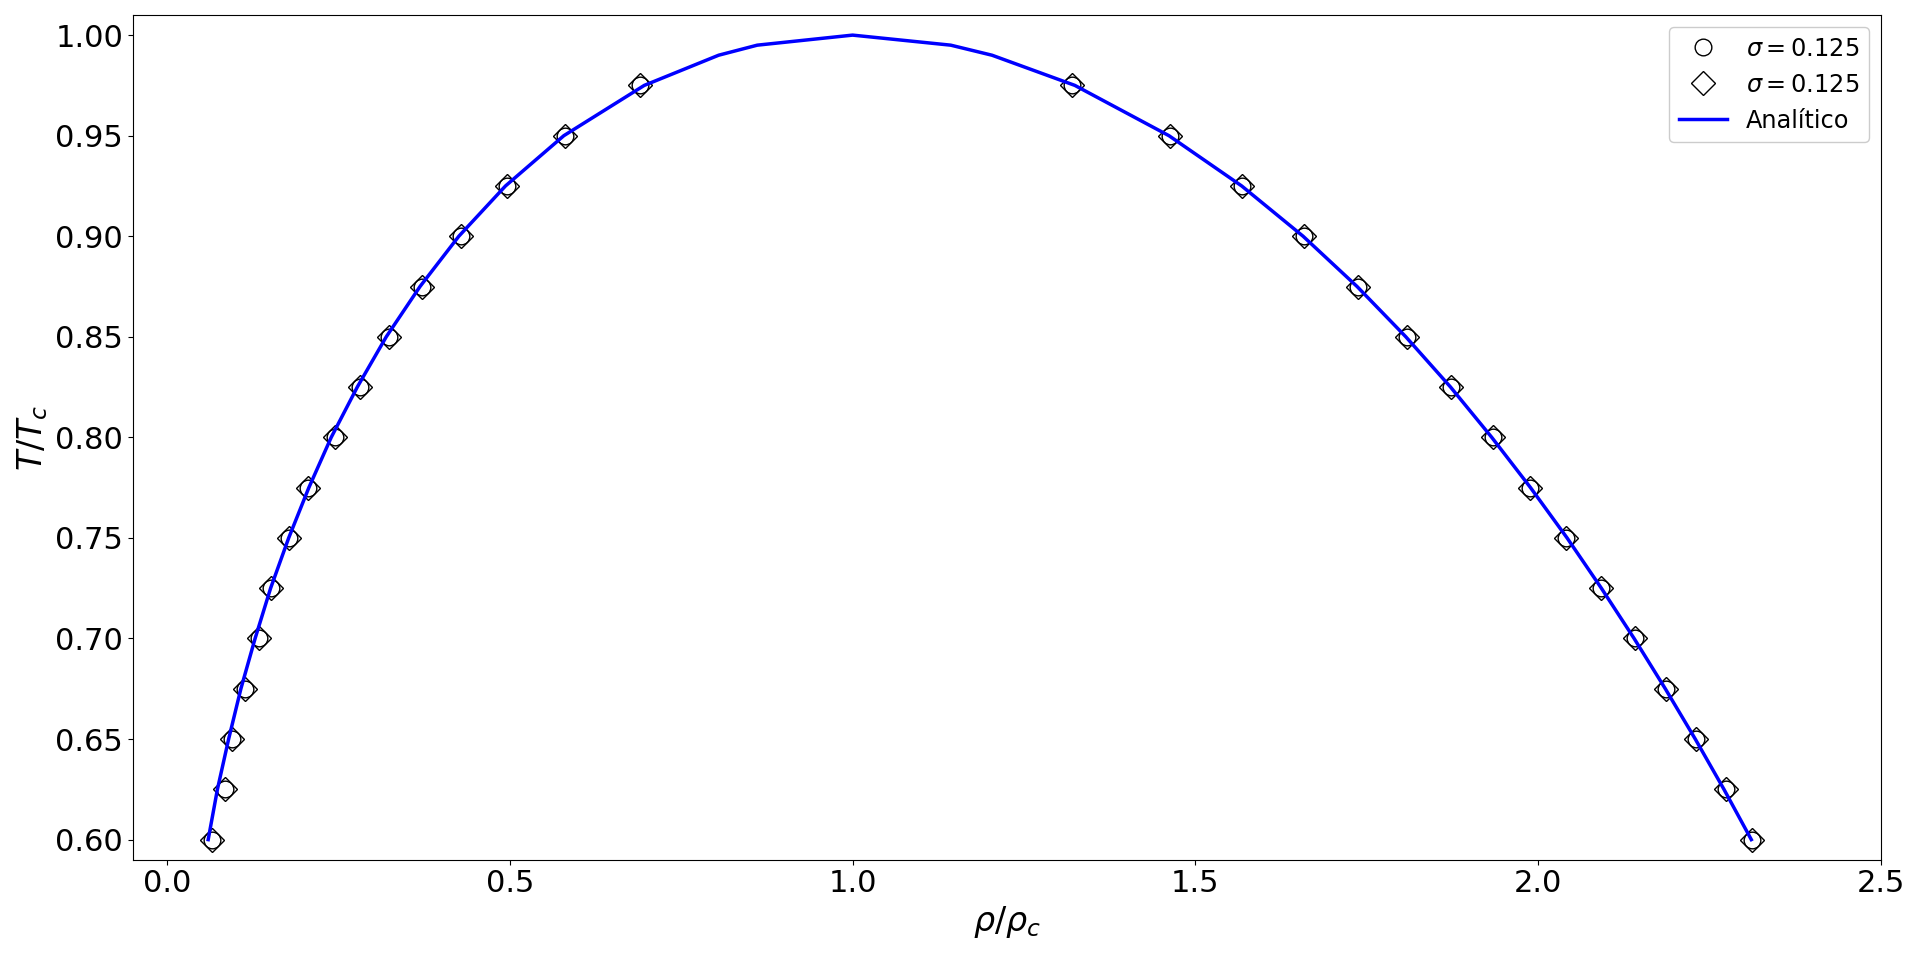
\includegraphics[width=\textwidth]{figs/cap4/v_760_MxC_c_comparacion}
	\caption{Curva de coexistencia de fases para un fluido de VdW con los parámetros $a = 0,5 $ y $b = 4,0 $, obtenida en simple precisión[$\bigcirc$] y doble precisión [$\diamondsuit$] en la GPU NVIDIA GeForce GTX 760 en el código desarrollado en \textsc{C}.} 
	\label{fig:v_760_MxC_c_comparacion}	
\end{figure}


%La Tabla (\ref{tab:comp_MxC_precisiones_10}) contiene los valores de las densidades de coexistencia: analítico, y los obtenidos mediante el código en simple precisión y doble precisión. De la Figura (\ref{fig:v_760_MxC_c_comparacion}) se observa que se ajusta mejor al resultado analítico la fase líquida que la fase gaseosa, por ello la Tabla (\ref{tab:comp_MxC_precisiones_10}) presenta esta diferenciación.

Para dar una idea de proximidad a la solución analítica se adoptó como parámetro la distancia entre los vectores de densidad de fase obtenido y el analítico. La distancia se calculó por medio de la Norma Euclídea, siendo calculada la distancia entre dos vectores \textbf{\textit{A}} y \textbf{\textit{B}} con \textit{i} elementos como indica la Ec.(\ref{eq:norma_euclidea}):

\begin{align}
dist(\mathbf{A},\mathbf{B}) = \sqrt{\sum_i {\left( a_i - b_i \right)}^2  }
\label{eq:norma_euclidea}
\end{align}

%A partir de los resultados obtenidos, que muestra la Tabla (\ref{tab:comp_MxC_precisiones_10}) en cuanto a la distancia de los vectores se observa que en doble precisión los resultados se aproximan mejor en la densidad de coexistencia de la fases, en la fase gaseosa; mientras que para la densidad de coexistencia de fase, de la fase líquida, se aproxima mejor mediante simple precisión. 

La mayor diferencia porcentual hallada para la distancia en la fase gaseosa, es que en simple precisión es 0,0034 \% mayor que en doble precisión. Para la fase líquida se obtuvo que en doble precisión es 0,0491 \% mayor la distancia que en simple precisión.


%% Please add the following required packages to your document preamble:
% \usepackage{multirow}
\begin{table}[h!]
\centering
%\resizebox{17cm}{!}{
	\begin{tabular}{|c|c|c|c|c|c|c|}
	\hline
	& \multicolumn{3}{c|}{${\rho_{r}}_{\>gaseoso}$}      & \multicolumn{3}{c|}{${\rho_{r}}_{\>líquido}$} \\ \hline
	$\mathbf{T_r}$    & \textbf{Analítico}      & \textbf{Simple}       & \textbf{Doble}     & \textbf{Analítico}      & \textbf{Simple}     & \textbf{Doble}   \\ \hline
	0.600 & 0.0599097 & 0.0653772 & 0.0653724 & 1.32424  & 1.31956 & 1.31975 \\ \hline
	0.625 & 0.0733723 & 0.0848112 & 0.0847656 & 1.46149  & 1.46239 & 1.4624  \\ \hline
	0.650 & 0.0897449 & 0.0951336 & 0.095124  & 1.56762  & 1.56858 & 1.56859 \\ \hline
	0.675 & 0.107606  & 0.113153  & 0.113147  & 1.56762  & 1.65819 & 1.65821 \\ \hline
	0.700 & 0.128332  & 0.13353   & 0.133511  & 1.6572   & 1.73703 & 1.73704 \\ \hline
	0.725 & 0.150966  & 0.15182   & 0.151811  & 1.73595  & 1.80812 & 1.80813 \\ \hline
	0.750 & 0.177353  & 0.177323  & 0.177319  & 1.80706  & 1.87326 & 1.87328 \\ \hline
	0.775 & 0.206739  & 0.206086  & 0.206075  & 1.87233  & 1.93364 & 1.93364 \\ \hline
	0.800 & 0.23938   & 0.244229  & 0.244223  & 1.93243  & 1.98754 & 1.98759 \\ \hline
	0.825 & 0.277393  & 0.281299  & 0.281284  & 1.98899  & 2.04083 & 2.04085 \\ \hline
	0.850 & 0.319677  & 0.323471  & 0.323456  & 2.0423   & 2.09124 & 2.09124 \\ \hline
	0.875 & 0.368925  & 0.371915  & 0.371891  & 2.09234  & 2.14114 & 2.14117 \\ \hline
	0.900 & 0.425549  & 0.428416  & 0.428335  & 2.14012  & 2.18665 & 2.18665 \\ \hline
	0.925 & 0.493618  & 0.495973  & 0.495947  & 2.18563  & 2.23017 & 2.23019 \\ \hline
	0.950 & 0.493618  & 0.580402  & 0.580368  & 2.22933  & 2.27407 & 2.27411 \\ \hline
	0.975 & 0.578746  & 0.690126  & 0.690247  & 2.27117  & 2.312   & 2.312   \\ \hline
	\textbf{Distancia} & -         & 2.05233   & 2.05226   & -        & 0.14234 & 0.14241 \\ \hline
\end{tabular}%}
    \caption{Comparación de las precisiones con respecto a cuánto se acercan al valor analitico, tanto para doble, como simple precision, la norma utilizada para medir la distancia de los vectores es la norma  euclídea. Para el problema de la Construcción de Maxwell con la GPU NVIDIA Geforce GTX 760.}
    \label{tab:comp_MxC_precisiones_10}
    \end{table}



\newpage

\subsection{Speed Up}

En la presente sección se muestran las mejoras en el tiempo de cálculo realizados para el código de \textsc{C} y \textsc{Cuda C}. El índice \textit{Speed Up} (SU) calcula la mejora en el tiempo de calculo entre códigos y se calcula con la Ec.(\ref{eq:speedup}), siendo \textit{t} el tiempo de cálculo y \textit{p} significa comparación entre precisiones. La comparación se realizó en simple y doble precisión para las dos (2) PC detalladas en la Sec. (\ref{sec_pc}).
\begin{align}
	SU = \frac{t_{\>C}}{t_{\>Cuda \> C}} \qquad 	{SU}_p = \frac{t_{\>doble \> precisión}}{t_{\>simple \> precisión}} 
	\label{eq:speedup}
\end{align}
Para calcular el \textsc{SU} de éste problema, se tomó una $T_r$ fija y se varió el tamaño de la grilla, de manera que ésta siempre fuese cuadrada, respetando un número de nodos de potencia de 2 en los lados del cuadrado. La cantidad de \textit{thread blocks} que se utilizó para realizar la comparación en el código de \textsc{CUDA} fueron de potencia de 2.

\subsubsection{NVIDIA GeForce GTX 760}

Los tamaños de grilla que se utilizaron para realizar las pruebas de tiempo de ésta placa, tienen el rango de grilla de 16x16 nodos hasta 2048x2048 nodos. La cantidad de \textit{thread blocks} que se utilizó fueron de 1 a 512.

Las Figuras (\ref{fig:s_760_MxC_simple_1.0}) y (\ref{fig:s_760_MxC_double_1.0}) muestran el \textit{SU} obtenido en simple precisión y doble precisión respectivamente. El mejor resultado en ambos casos se obtuvo para un número de \textit{thread block} igual a 64, donde la mejora fue de 18.67 y 11.40 en simple y doble precisión respectivamente, para el mayor número de elementos de malla.


\begin{figure}[htbp]
	\centering
	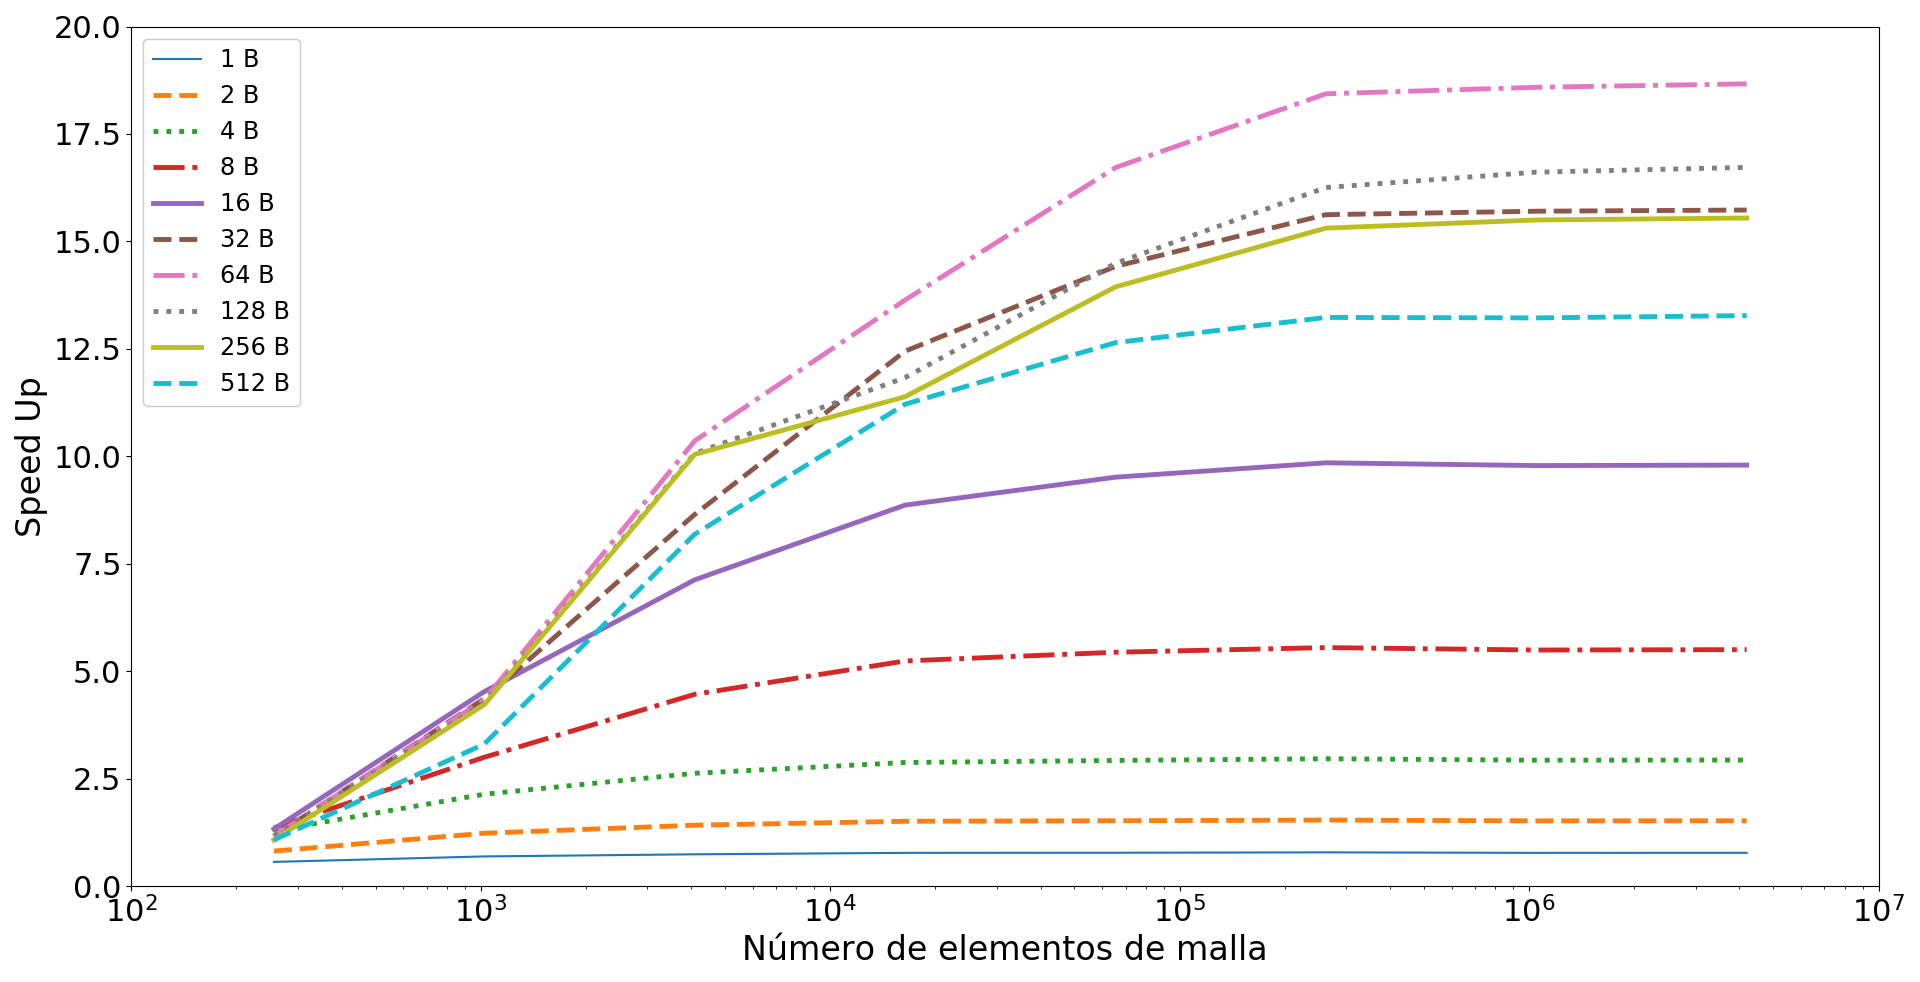
\includegraphics[width=\textwidth]{figs/cap4/s_760_MxC_simple_10}
	\caption{SU realizado para el problema de la Construcción de Maxwell en simple precisión con una CPU Intel Core i7-3770 y GPU NVIDIA GeForce GTX 760.} 
	\label{fig:s_760_MxC_simple_1.0}	
\end{figure}

\begin{figure}[htbp]
	\centering
	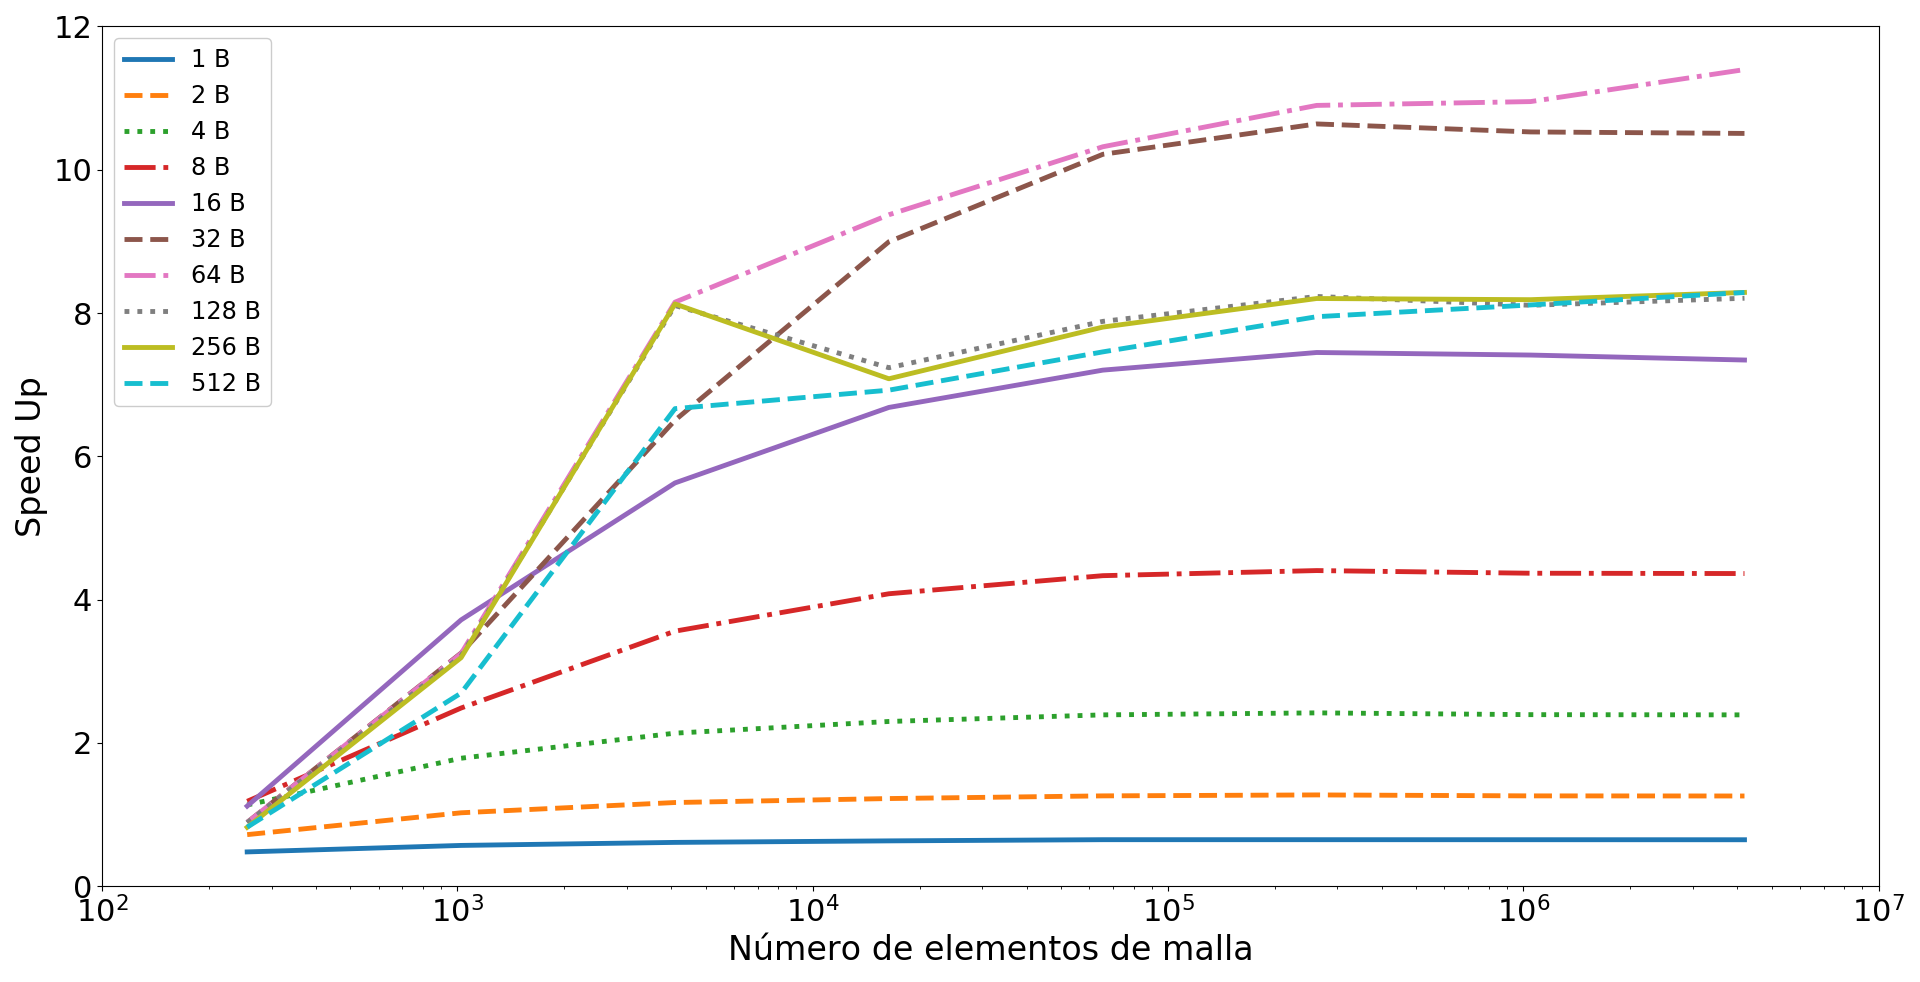
\includegraphics[width=\textwidth]{figs/cap4/s_760_MxC_double_10}
	\caption{SU realizado para el problema de la Construcción de Maxwell en doble precisión con una CPU Intel Core i7-3770 y GPU NVIDIA GeForce GTX 760.} 
	\label{fig:s_760_MxC_double_1.0}	
\end{figure}

\begin{figure}[h!]
	\centering
	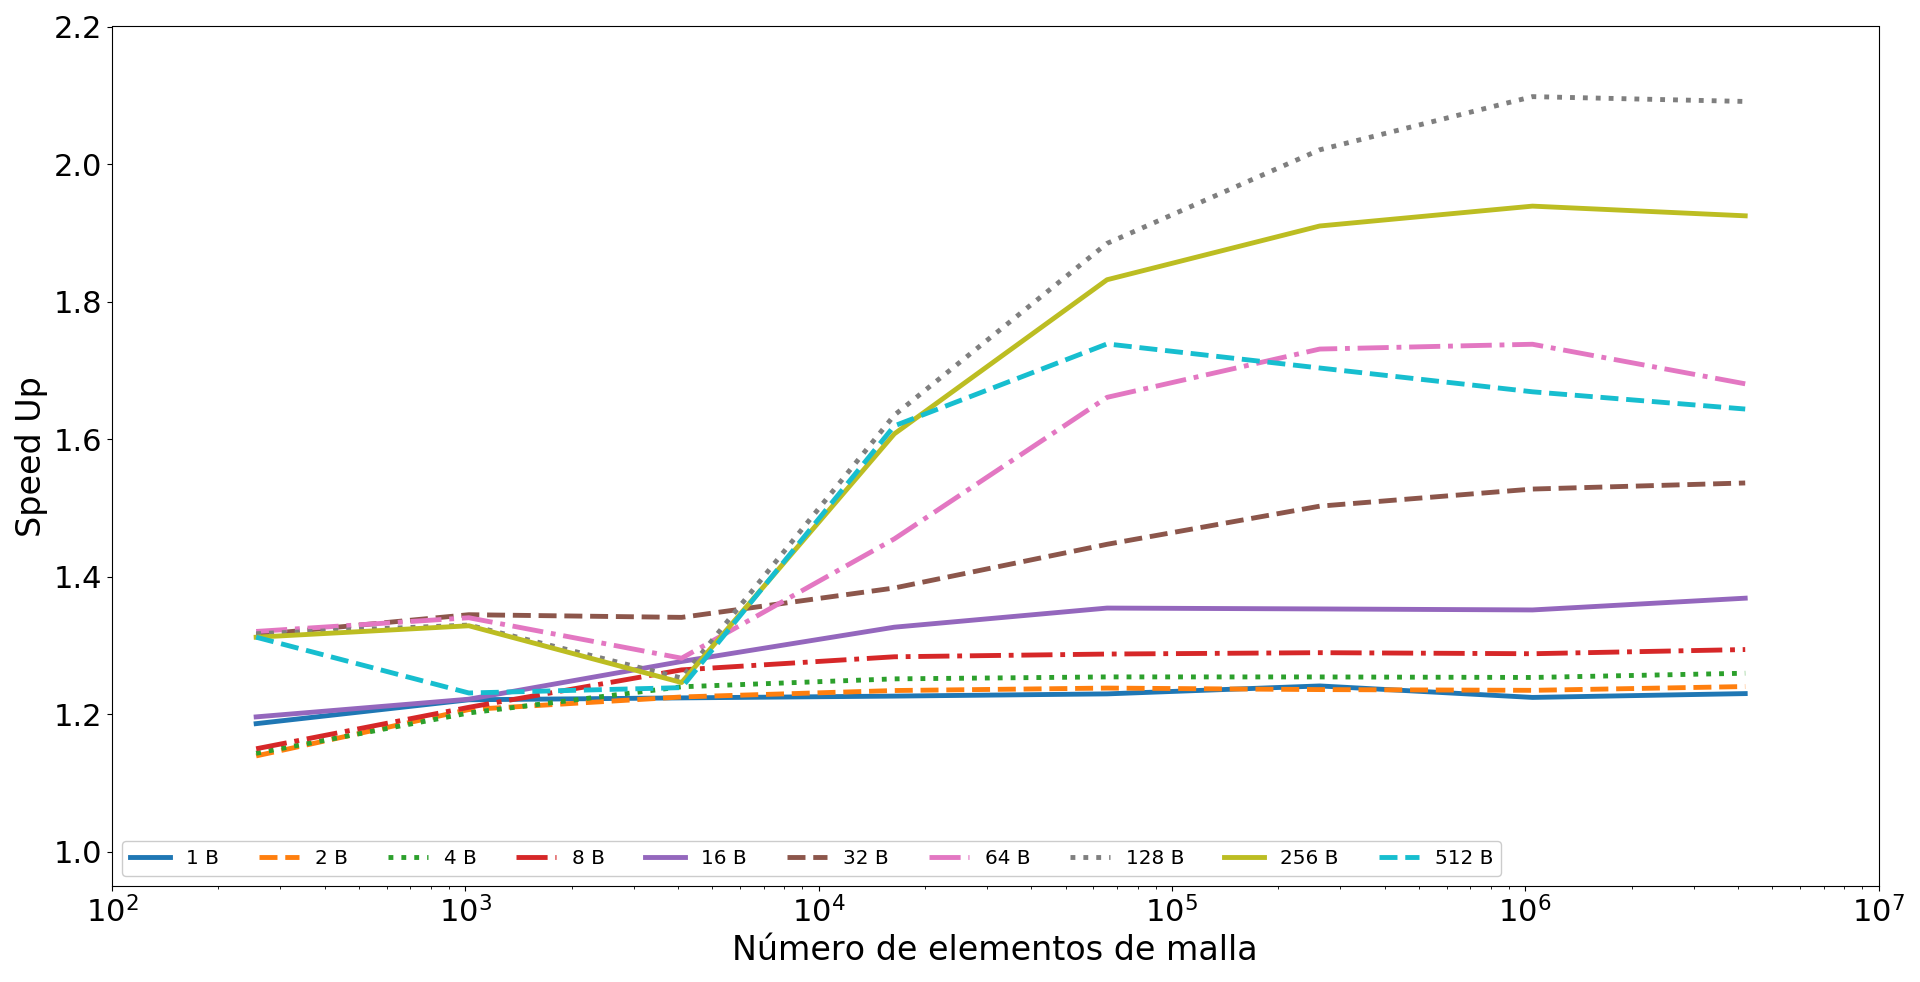
\includegraphics[width=\textwidth]{figs/cap4/c_760_MxC_cuda_10}
	\caption{$SU_p$ realizado para el problema de la Construcción de Maxwell en en el código de \textsc{Cuda C} con la GPU NVIDIA GeForce GTX 760.} 
	\label{fig:c_760_MxC_cuda_10}	
\end{figure}

La Figura (\ref{fig:c_760_MxC_cuda_10}) muestra el ${SU}_p$ del código de \textsc{Cuda C} en la GPU NVIDIA GeForce GTX 760. Para un número de \textit{thread block} igual a 64, el tiempo de cálculo en doble precisión es 1,68 veces mayor que en simple precisión en el mayor número de elementos de malla calculado. Se reporta únicamente el resultado para esa cantidad de \textit{thread block}, debido a que los resultados de las Figuras (\ref{fig:s_760_MxC_simple_1.0}) y (\ref{fig:s_760_MxC_double_1.0}) indican que es el que tiene un mayor SU.


\subsubsection{NVIDIA GeForce GTX 970}

Los tamaños de grilla que se utilizaron para realizar las pruebas de tiempo de ésta placa, tienen el rango de grilla de 16x16 nodos hasta 4096x4096 nodos en simple precisión y de 16x16 nodos hasta 2048x2048 nodos en doble precisión . La cantidad de \textit{thread blocks} que se utilizó fueron de 1 a 512.



\begin{figure}[htbp]
	\centering
	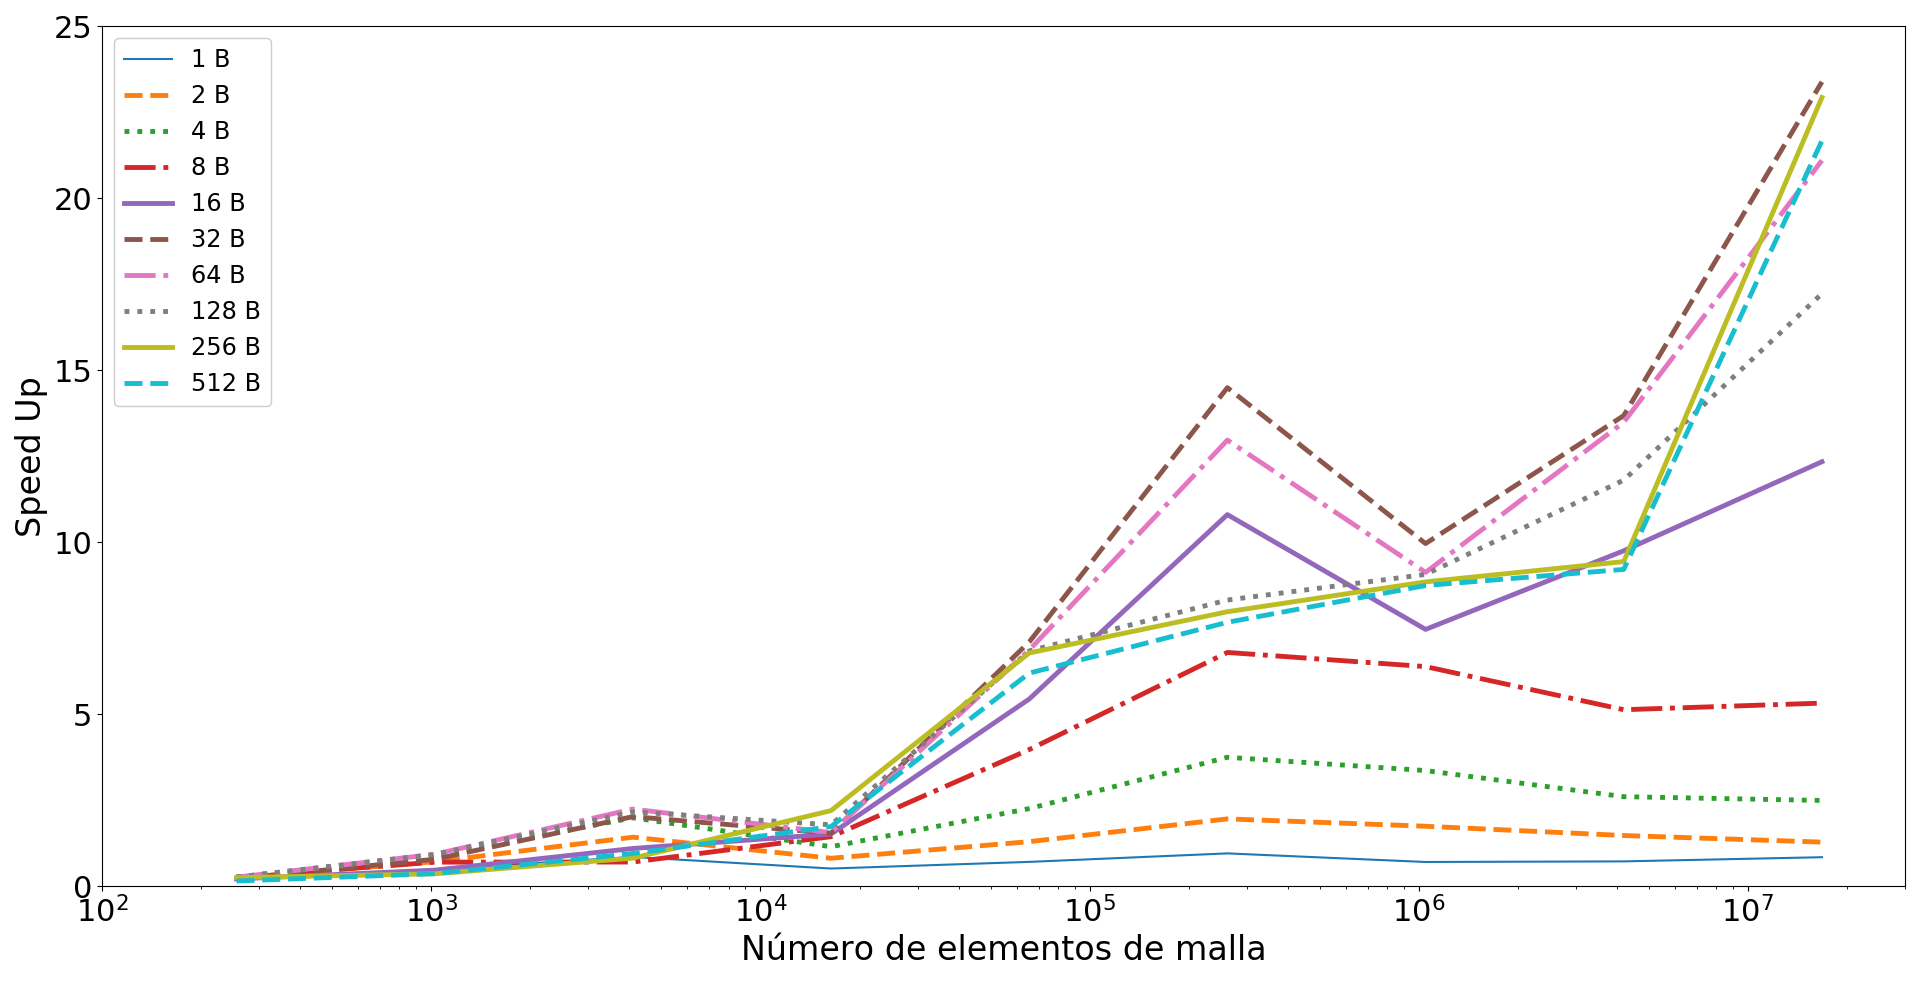
\includegraphics[width=0.99\textwidth]{figs/cap4/s_970_MxC_simple_10}
	\caption{SU realizado para el problema de la Construcción de Maxwell en simple precisión con una CPU Intel Core i7-4770 y GPU NVIDIA GeForce GTX 970.} 
	\label{fig:s_970_MxC_simple_10}	
\end{figure}

\begin{figure}[htbp]
	\centering
	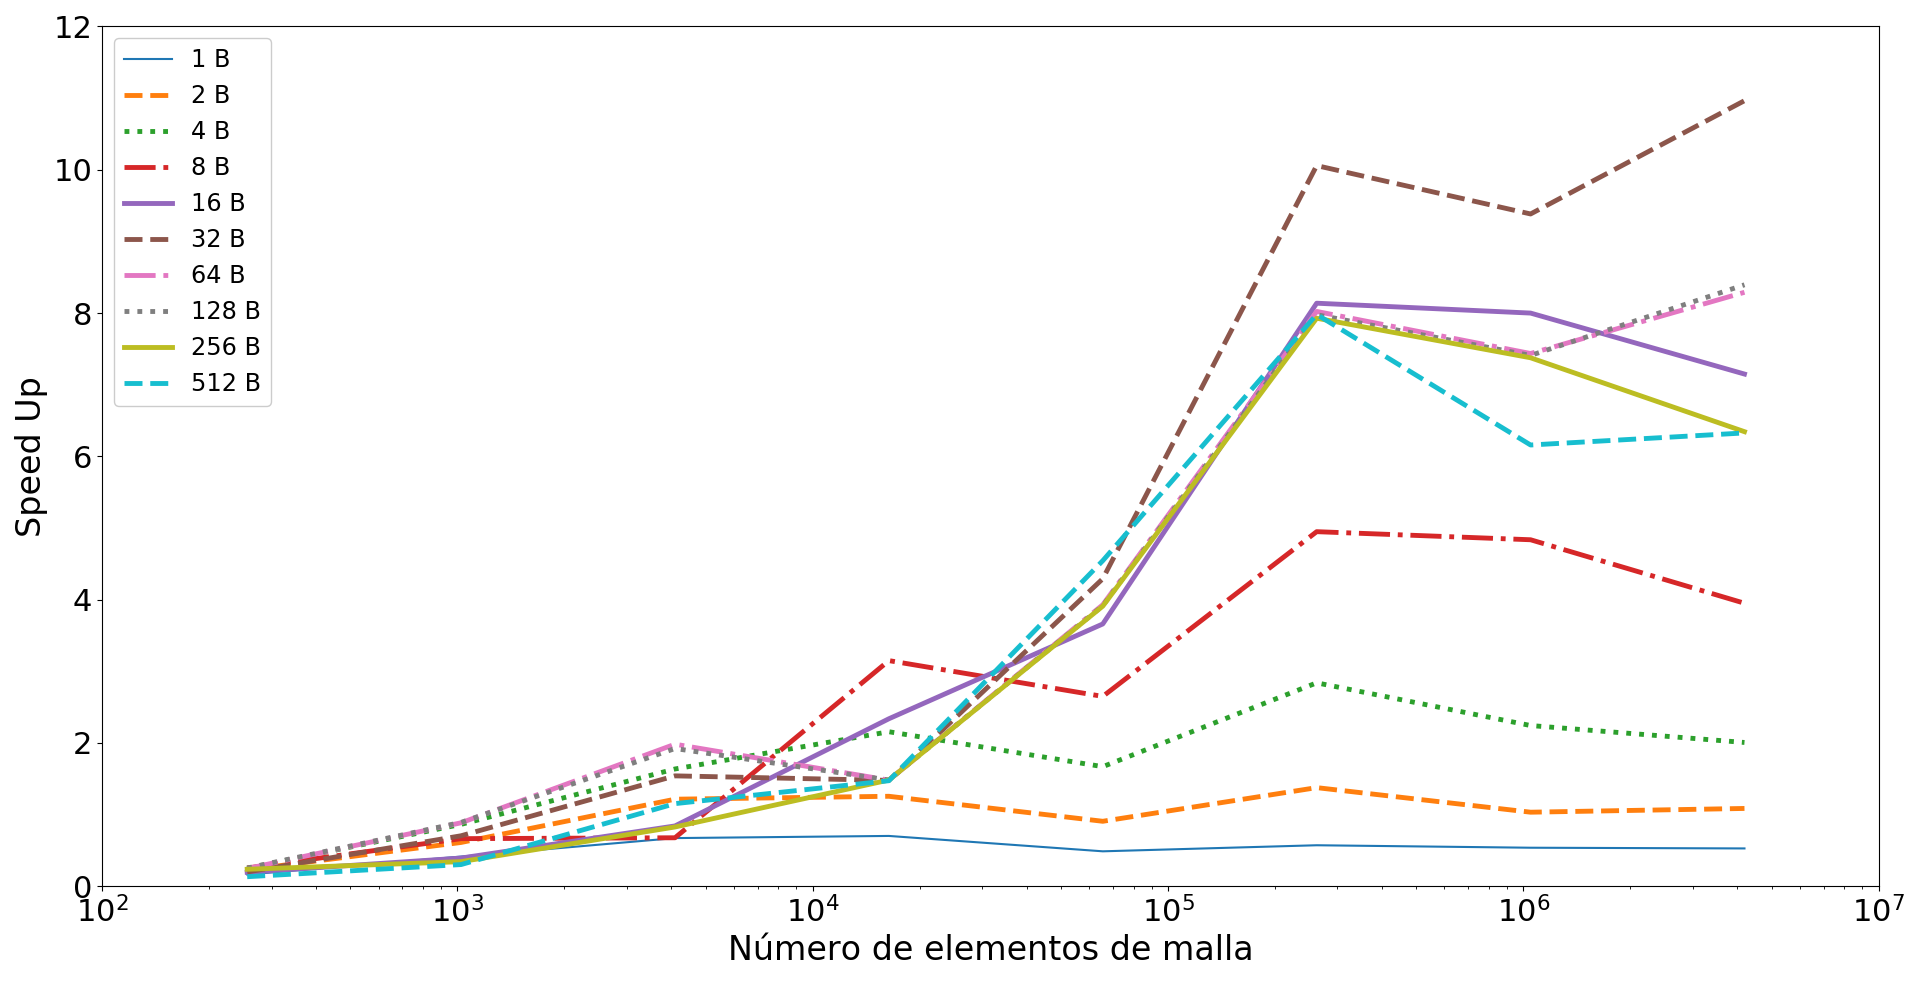
\includegraphics[width=0.99\textwidth]{figs/cap4/s_970_MxC_double_10}
	\caption{SU realizado para el problema de la Construcción de Maxwell en doble precisión con una CPU Intel Core i7-4770 y GPU NVIDIA GeForce GTX 970.} 
	\label{fig:s_970_MxC_double_10}	
\end{figure}

\newpage

Las Figuras (\ref{fig:s_970_MxC_simple_10}) y (\ref{fig:s_970_MxC_double_10}) muestran el \textit{SU} obtenido en simple precisión y doble precisión respectivamente. El mejor resultado en ambos casos se obtuvo para un número de \textit{thread block} igual a 32, donde la mejora fue de 23.39 y 10.96 en simple y doble precisión respectivamente, para el mayor número de elementos de malla.

La Figura (\ref{fig:c_970_MxC_cuda_10}) muestra el ${SU}_p$ del código de \textsc{Cuda C} en la GPU NVIDIA GeForce GTX 970. Para un número de \textit{thread block} igual a 32, el tiempo de cálculo en doble precisión es 1,29 veces mayor que en simple precisión en el mayor número de elementos de malla calculado. Se reporta únicamente el resultado para esa cantidad de \textit{thread block}, debido a que los resultados de las Figuras (\ref{fig:s_970_MxC_simple_10}) y (\ref{fig:s_970_MxC_double_10}) indican que es el que tiene un mayor SU.

\begin{figure}[htbp]
	\centering
	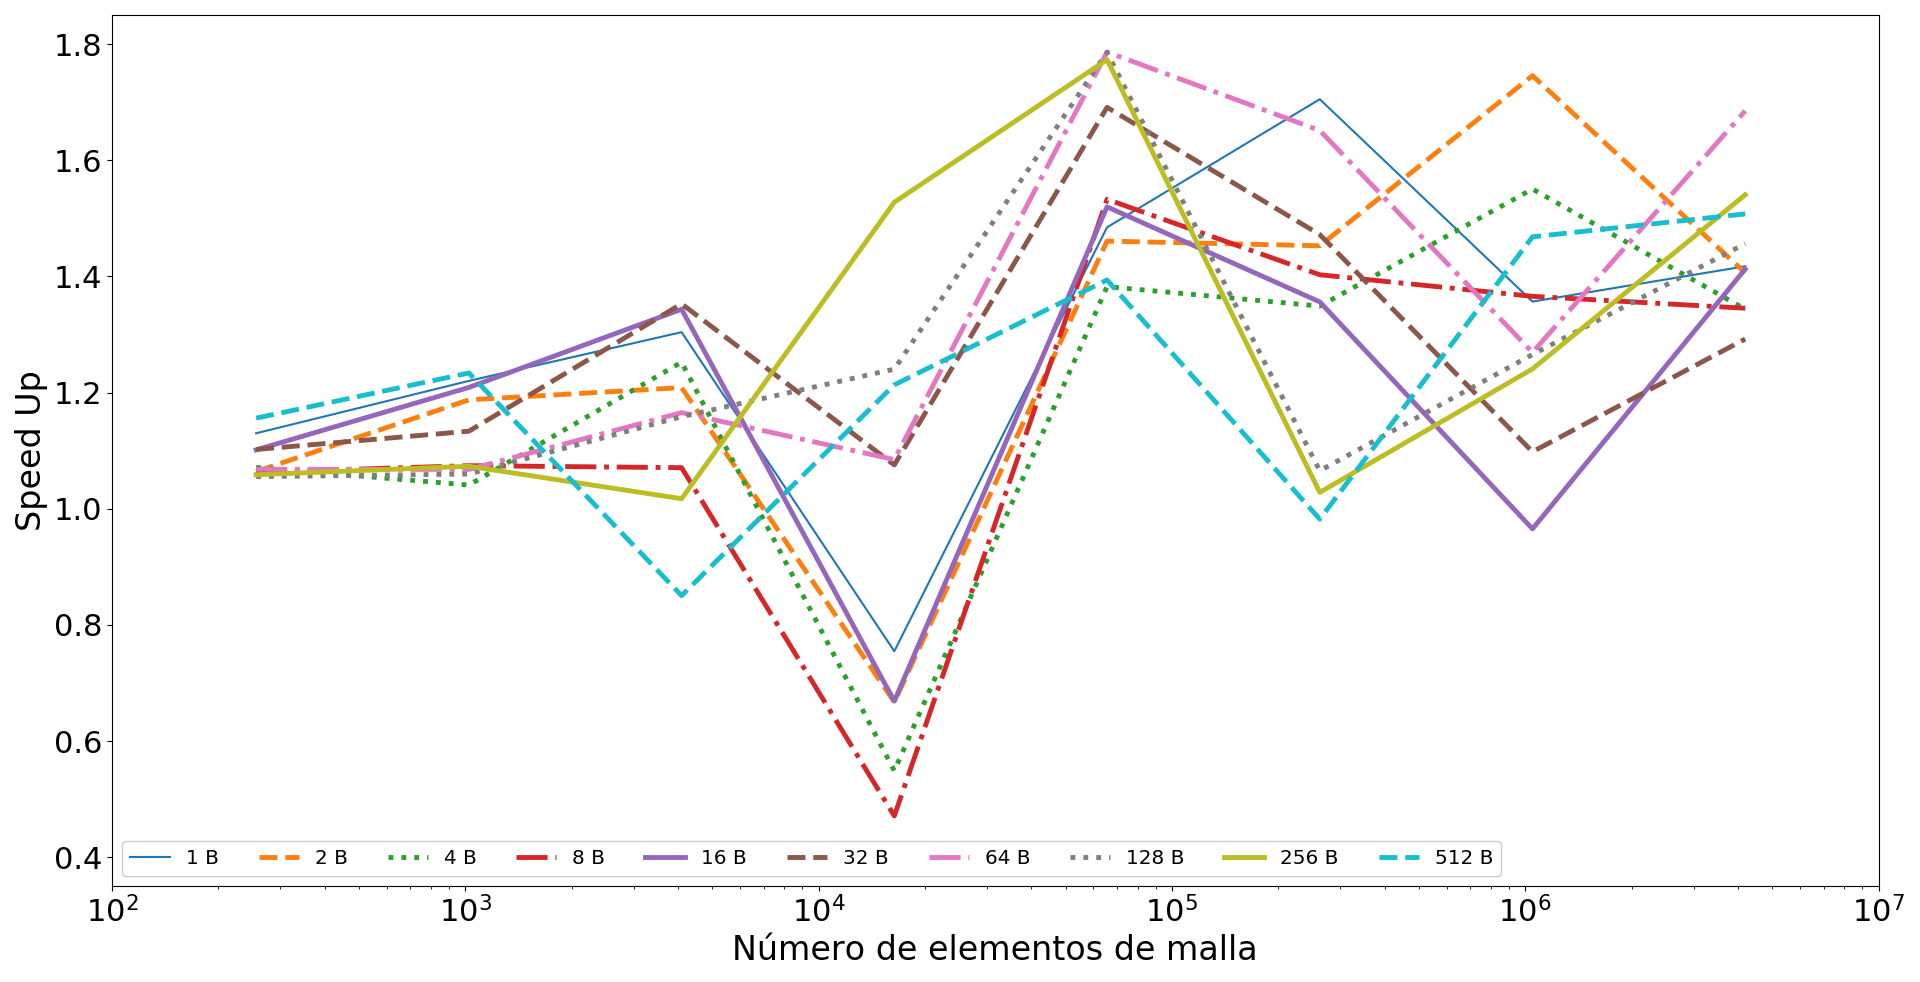
\includegraphics[width=\textwidth]{figs/cap4/c_970_MxC_cuda_10}
	\caption{$SU_p$ realizado para el problema de la Construcción de Maxwell en en el código de \textsc{Cuda C} con la GPU NVIDIA GeForce GTX 970.} 
	\label{fig:c_970_MxC_cuda_10}	
\end{figure}




Se puede concluir después de haber realizado un SU y $SU_p$ a las dos PC que se tuvo acceso para realizar el presente trabajo, de que la utilización de simple precisión en el código de \textsc{Cuda C} es más conveniente que doble precisión. Una de las razones es que no hay demasiada diferencia entre los valores que se pueden obtener, según los resultados obtenidos no difirieren más del 0,003 \%. Otra de las razones es que debido a las mejoras obtenidas en los tiempos de cálculo en las placas NVIDIA GeForce GTX 760 y NVIDIA GeForce GTX 970 en el código de \textsc{Cuda C} de 18.67 y 23.39 respectivamente en simple precisión que el código de \textsc{C}. Las mejoras en doble precisión de las ganancias son de 11.40 y 10.96 respectivamente en las placas mencionadas. Por lo que el resultado obtenido en simple precisión difiere apenas un 0.003 \% que en doble precisión, además siendo 1.68 y 1.29 veces más rapido según la GPU utilizada.

\newpage

\section{Estratificación de un fluido VdW con temperatura no uniforme}

\begin{figure}[htbp]
	\centering
	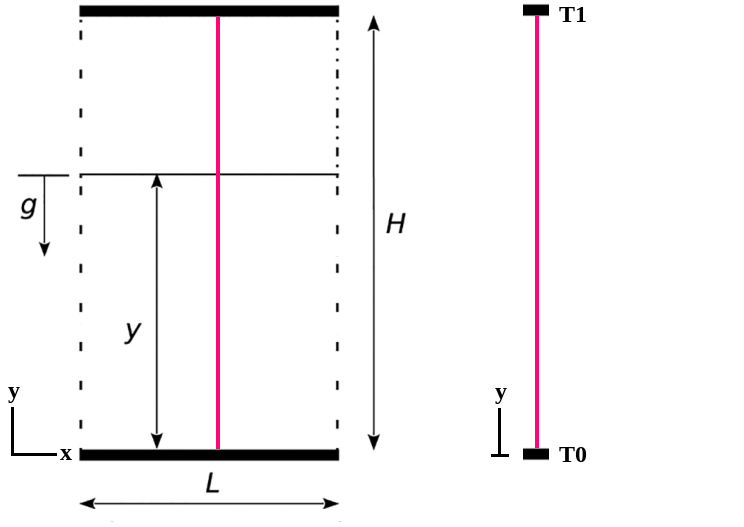
\includegraphics[width=0.3\textwidth]{figs/cap4/esquema_problema_VdW}
	\caption{Esquema del problema de la estratificación de un fluido VdW. Donde se muestra el alto (H) de la cavidad y el ancho (L).} 
	\label{fig:esquema_VdW}	
\end{figure}

Se quiere resolver el problema de una cavidad unidimensional en presencia de un fluido cuya EOS es la de Van der Waals; con temperatura  no uniforme y fuerza de gravedad no nula. Éste problema fue desarrollado por Berberan-Santos \cite{berberan2002liquid} y que Fogliatto \cite{fogliatto2019simulation} extendió. En éste caso se resuelven las dos ecuaciones pseudo-potencial del LBM, la ecuación hidrodinámica y la ecuación de energía.

Se toma como coordenada del problema \textit{y}, teniéndose una temperatura fija $T_{0}$ en $y = 0$ y $T_{1}$ en $y = H$ como se observa en la Figura (\ref{fig:esquema_VdW}) en presencia de la gravedad.

El gradiente de presión surge de realizar el balance de momento en un volumen diferencial, obteniéndose:

\begin{align}
	\frac{d P}{d y} = - g M C(y)
\end{align}

siendo \textit{g} la gravedad, \textit{M} el peso molecular, $C = \frac{1}{v}$ la fracción molar, \textit{v} el volumen molar y \textit{P} la presión.

Realizando la adimensionalización de $ P_r = \frac{P}{P_c}$ , $ T_r = \frac{T}{T_c}$, $c = C v_c$ y $E_r = \frac{M g y}{R T_c}$; siendo \textit{c} el punto crítico en el cuál comienza la coexistencia de las dos fases, se pueden reemplazar en el gradiente de presión y una Ecuación de estado para obtener una ecuación adimensional con la concentración molar distribuida \cite{fogliatto2019simulation}.



Al elejir la EOS de VdW de la Ec.(\ref{eq:VdW_P}), se obtiene la siguiente ecuación adimensional diferencial:

\begin{align}
	\frac{d c}{d E_r} = - \left[ c + \frac{d T_r}{d E_r} \left( \frac{c}{1 - \frac{c}{3}}\right) \right] \left[	\frac{1}{\frac{T_r}{{\left(1- \frac{c}{3}\right)}^2} - \frac{9}{4} c}  \right] 
	\label{eq:adim_dif}
\end{align} 

donde la posición de la interface dentro de la cavidad se puede determinar utilizando la masa inicial, siendo la misma una condición inicial para realizar la integración de la Ec. (\ref{eq:adim_dif}). Si se elije  resolver iterativamente la Ec. (\ref{eq:adim_dif}) junto con la ecuación macroscópica Ec. (\ref{eq:calor_ecu}) (ecuación del calor) se puede obtener las distribuciones de densidad y temperatura de la cavidad \cite{fogliatto2019simulation}. A partir de la densidad y temperatura recuperadas, se obtienen dos curvas adimensionales correspondientes al perfil de temperatura y al de concentraciones. 

En éste problema a validar, se toma como temperatura fija $T_1 = 0.99 \> T_c$, y se hace variar el valor de  $T_0$. Se asigna la siguiente nomenclatura $\rho_r = \frac{\rho}{\rho_c}$ y  $Y_r = \frac{y}{H}$. En las Figuras (\ref{fig:v_760_VdW_c_simple_rho_y}) y (\ref{fig:v_760_VdW_c_simple_T_y}) se muestran las curvas adimensionales de $ \rho_r - Y_r $ y $ T_r - Y_r $ respectivamente.

%\begin{figure}[htbp]
%	\centering
%	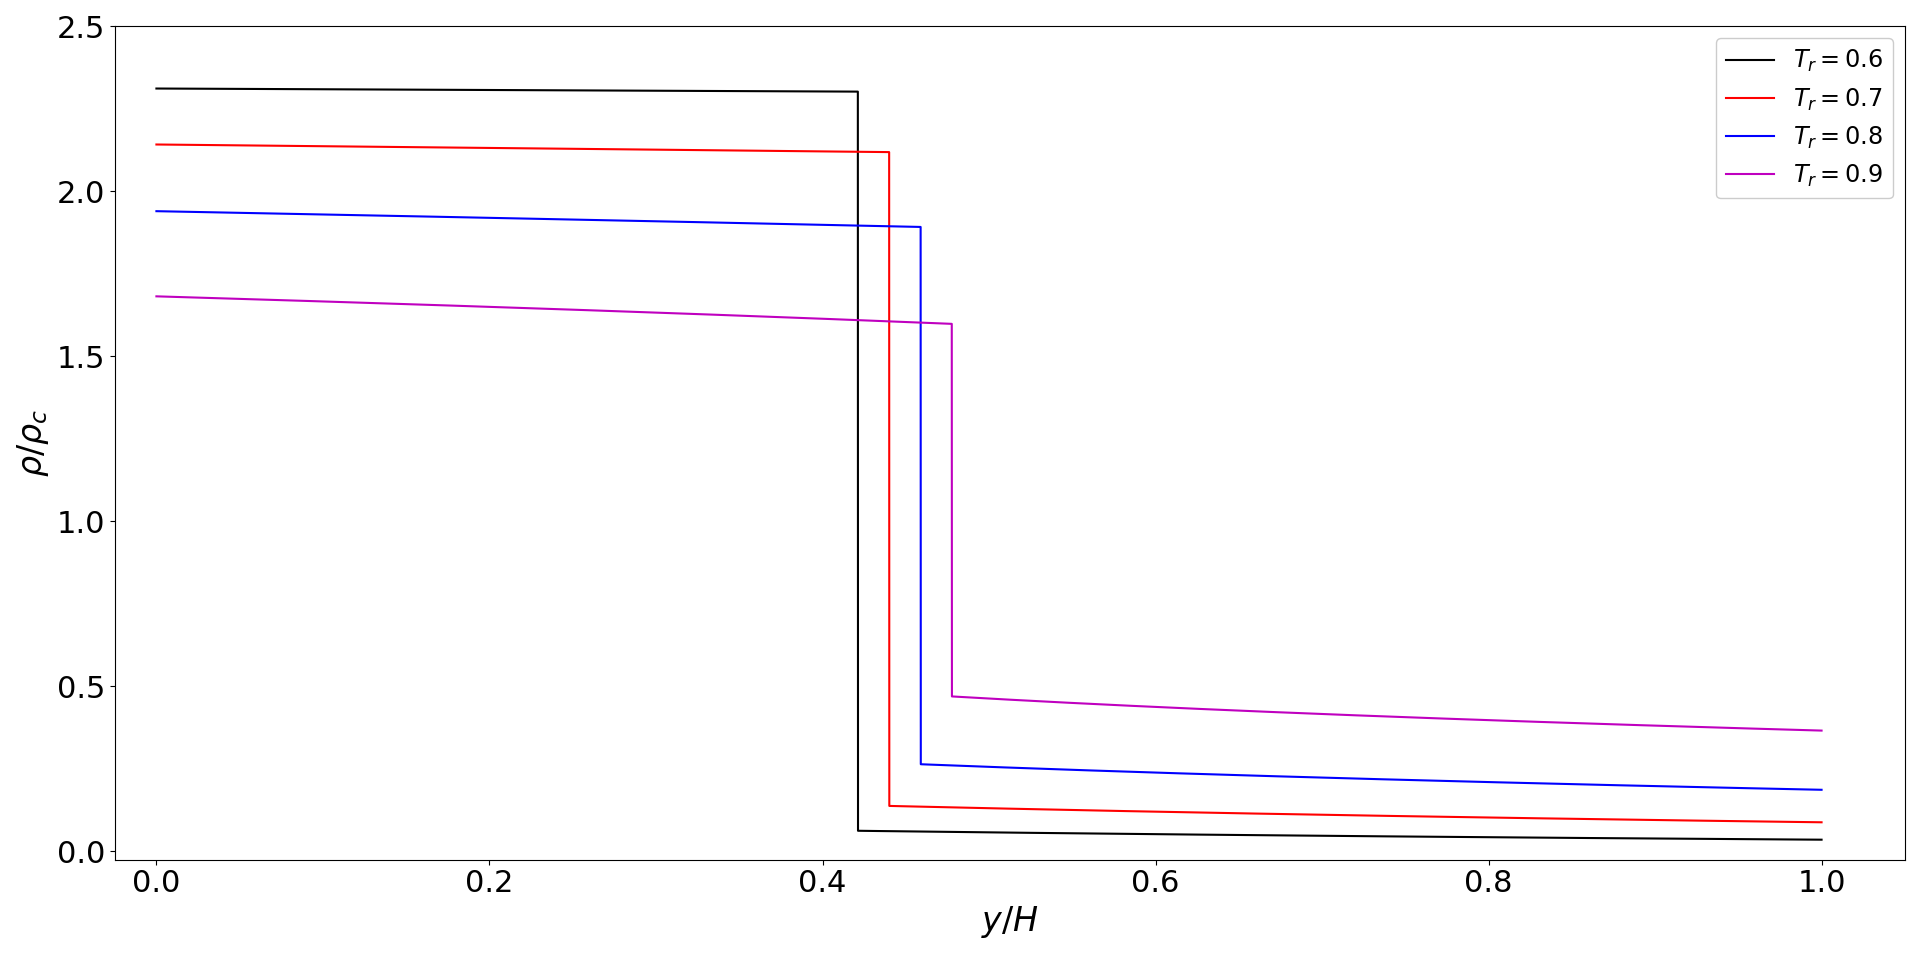
\includegraphics[width=\textwidth]{figs/cap4/VdW_val_rho_y}
%	\caption{Perfil de densidad adimensional a lo largo de la longitud de la pared,para distintos valores de condición de temperatura fija en $y = 0$, para un fluido de VdW con los parámetros $a = 0,5 $ y $b = 4,0 $, obtenida en simple precisión en la GPU NVIDIA GeForce GTX 760 en el código desarrollado en \textsc{C}.} 
%	\label{fig:VdW_val_rho_y}	
%\end{figure}
%
%\begin{figure}[htbp]
%	\centering
%	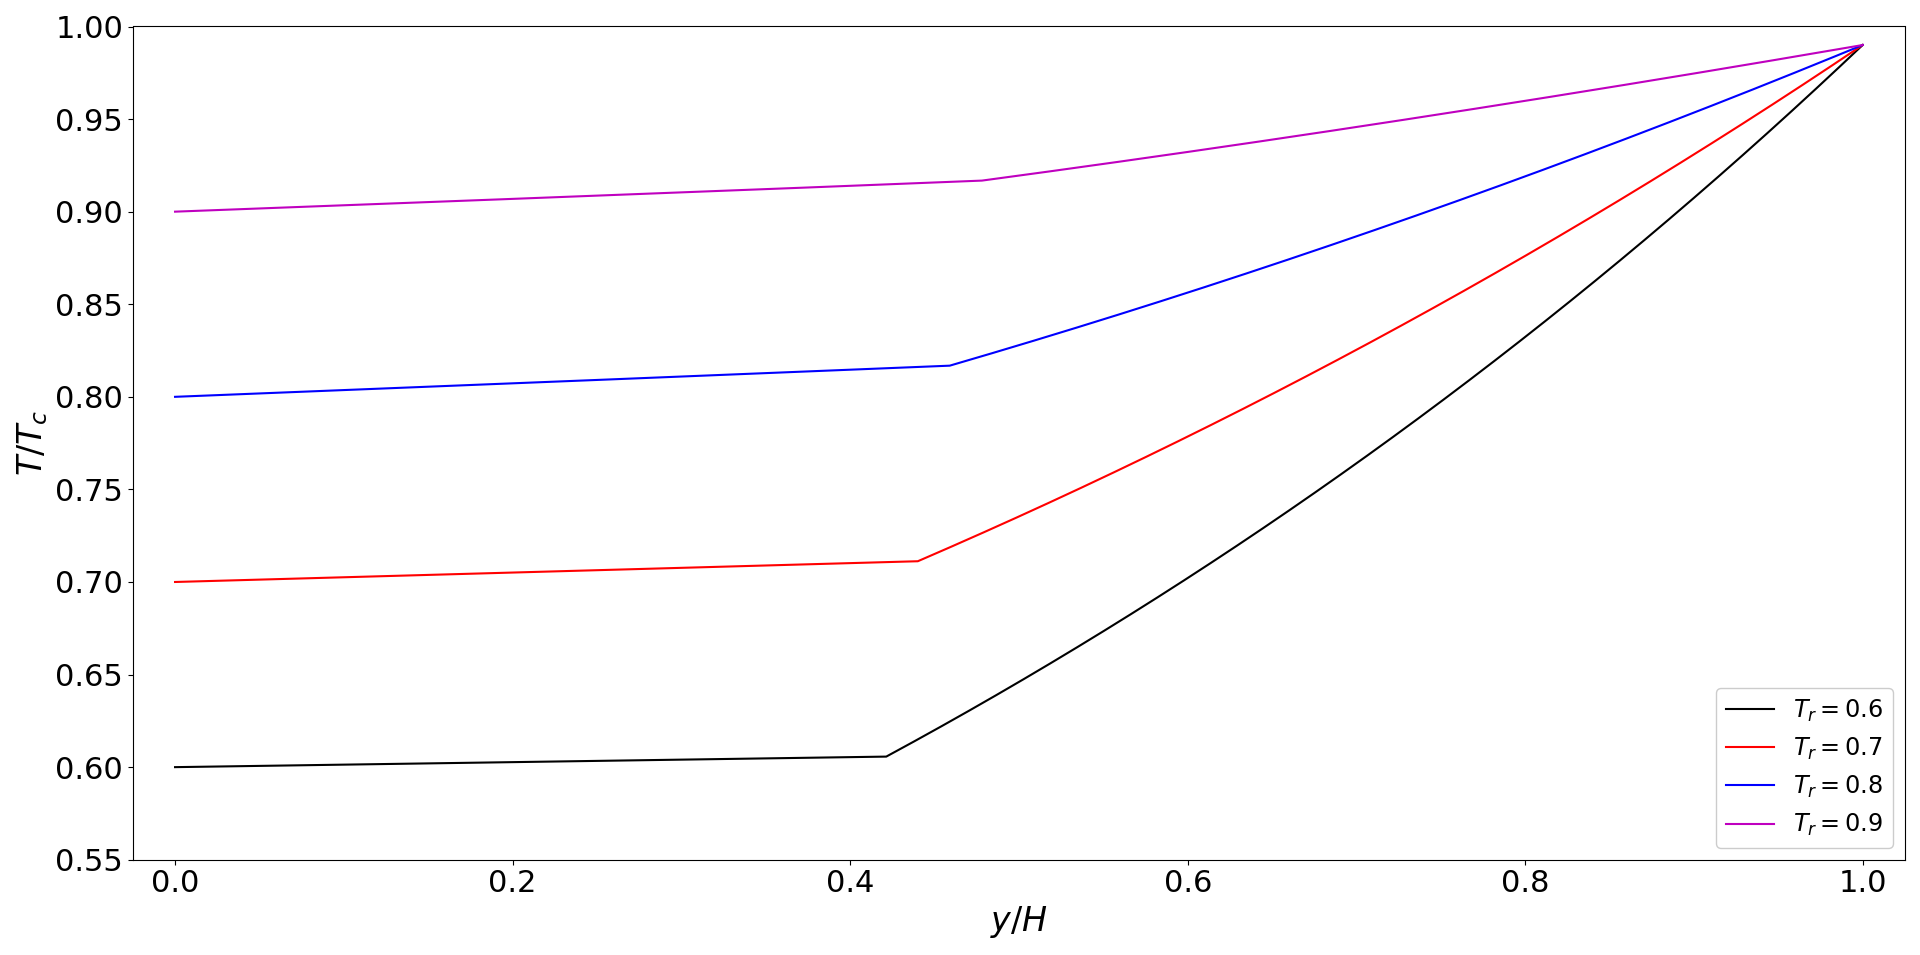
\includegraphics[width=\textwidth]{figs/cap4/VdW_val_T_y}
%	\caption{Perfil de temperatura adimensional a lo largo de la longitud de la pared, para distintos valores de condición de temperatura fija en $y = 0$,para un fluido de VdW con los parámetros $a = 0,5 $ y $b = 4,0 $, obtenida en simple precisión en la GPU NVIDIA GeForce GTX 760 en el código desarrollado en \textsc{C}.} 
%	\label{fig:VdW_val_T_y}	
%\end{figure}



\subsection{Validación}

La validación de éste problema se hizo utilizando los parámetros $a =0,5$ y $b = 4,0$; para un tamaño de malla de 3 x 300 nodos y $T_0 = T_r$, variando $T_r$ con un paso de $0,025$ en el rango de $[0,6 - 0,975]$, donde se muestra en los gráficos únicamente los valores de $T_r = 0,6 ; 0,7 ; 0,8 \> y \> 0,9$.  Los parámetros de LBM son los que se detallan a continuación:
\begin{align*}
diag(\mathbf{\Lambda}) = 
\begin{bmatrix}
1.0 & 0.8 & 1.1 & 1.0 & 1.1 & 1.0 & 1.1 & 0.8 & 0.8 \\
\end{bmatrix}\\
diag(\mathbf{Q}) = 
\begin{bmatrix}
1.0 & 1.0 & 1.0 & 0.8 & 1.0 & 0.8 & 1.0 & 1.0 & 1.0 \\
\end{bmatrix}\\
\alpha_{1} = 1.0 \qquad 	\alpha_{2} = 1.0 \qquad C_{v} = 1.0\\
G = -1.0 \quad c = 1.0 \quad \sigma = 0.125 \quad a = 0.5 \quad b = 4.0 \\
\mathbf{g} = (0.0 \quad-1.234567e^{-7}\quad 0.0 ) \qquad \rho_c = \frac{1}{12} \qquad T_c = 0.037037037
\end{align*}


La Figura(\ref{fig:v_760_VdW_c_simple_rho_y}) y (\ref{fig:v_760_VdW_c_simple_T_y})  muestran la validación del código realizado en \textsc{C} para simple precisión en una GPU NVIDIA GeForce GTX 760; con distintos valores de $T_0$. 

El quiebre abrupto y discontínuo de la densidad a lo largo de la pared en la Figura (\ref{fig:v_760_VdW_c_simple_rho_y}) muestra la coexistencia de las dos fases, para la solución analítica. Debido a que se tiene una solución continua y difusa porque el modelo toma una cierta cantidad de nodos como separación entre ambas fases, se presenta una mayor diferencia en el ajuste de la curva obtenida con la analítica en el cambio de fase. Lo mismo sucede en la Figura (\ref{fig:v_760_VdW_c_simple_T_y}). El paso de tiempo utilizado en cada uno de los nodos de la malla fue de 750000. El resultado obtenido para ambas curvas validades es similar en primer orden en el código de \textsc{C} y \textsc{Cuda C}.

\begin{figure}[h!]
	\centering
	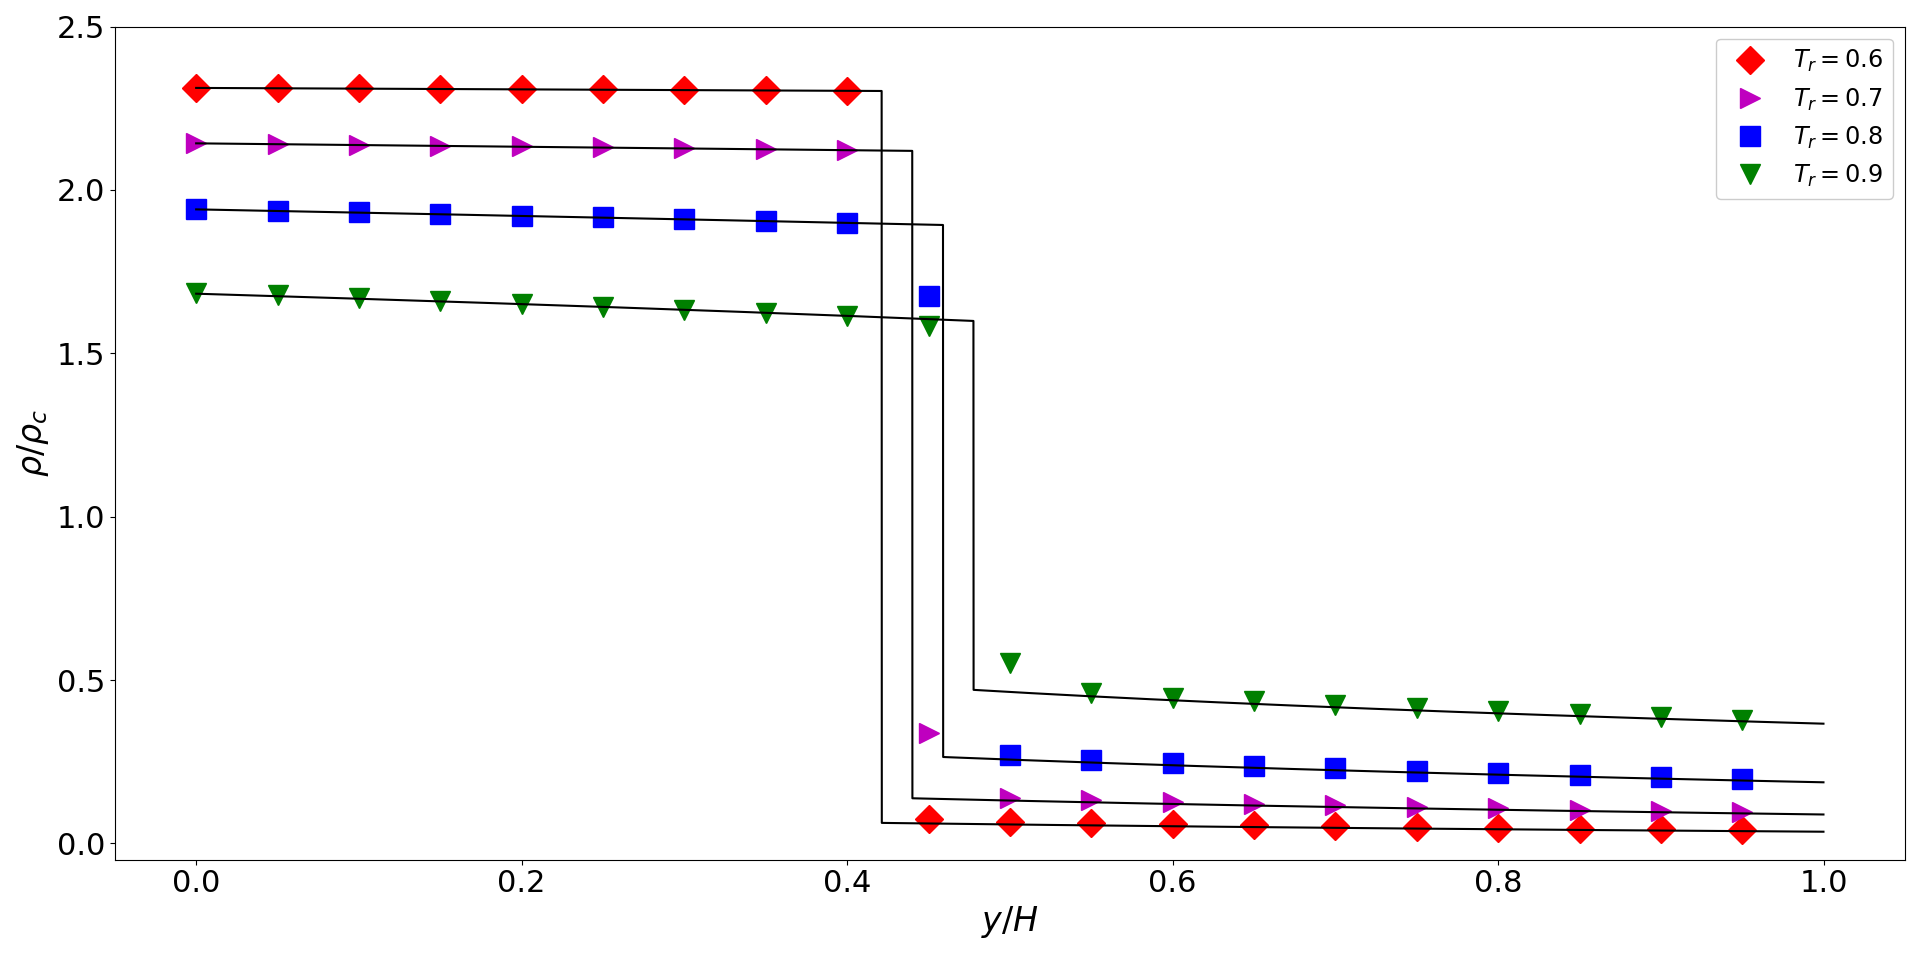
\includegraphics[width=\textwidth]{figs/cap4/v_760_VdW_c_simple_rho_y}
	\caption{Perfil de densidad adimensional a lo largo de la cavidad, para valores de $T_0 = T_r$ , siendo $T_r = 0,6 ; 0,7 ; 0,8 y 0,9$, para un fluido de VdW con los parámetros $a = 0,5 $ y $b = 4,0 $, obtenida en simple precisión en la GPU NVIDIA GeForce GTX 760 en el código desarrollado en \textsc{C}.}
	\label{fig:v_760_VdW_c_simple_rho_y}	
\end{figure}

\begin{figure}[h!]
	\centering
	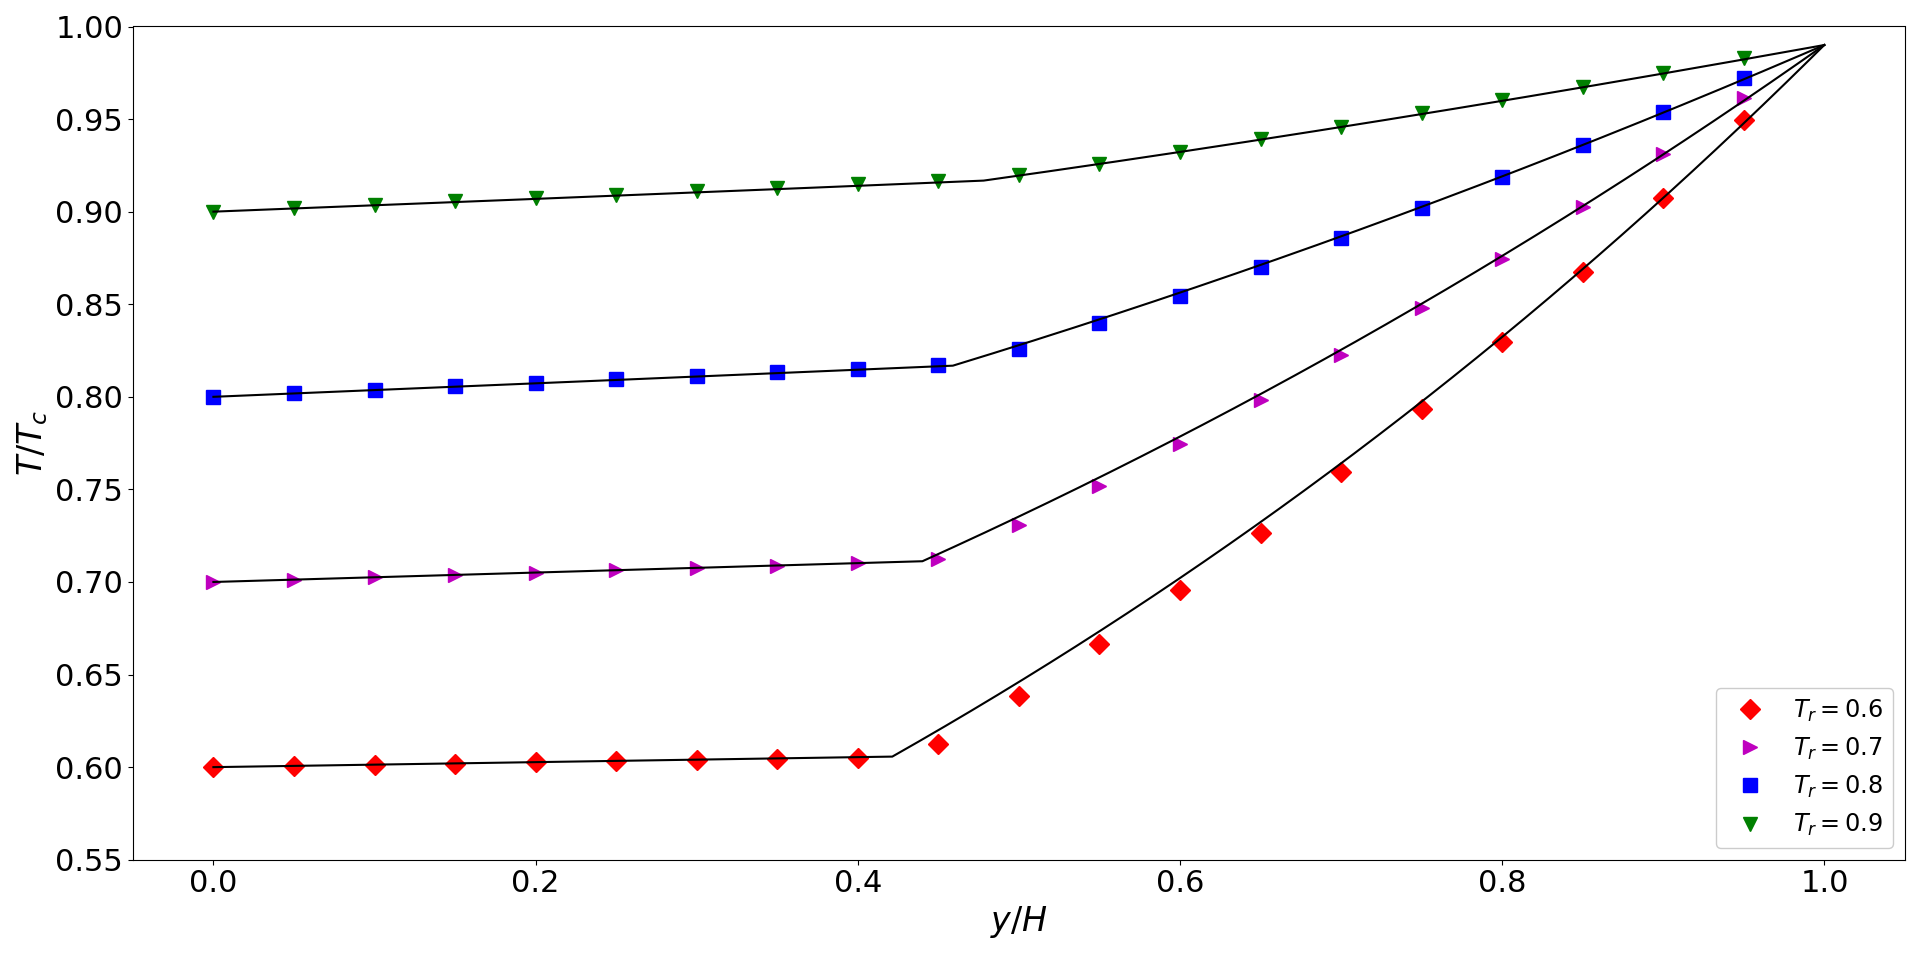
\includegraphics[width=\textwidth]{figs/cap4/v_760_VdW_c_simple_T_y}
	\caption{Perfil de temperatura adimensional a lo largo de la cavidad de la pared, para valores de $T_0 = T_r$ , siendo $T_r = 0,6 ; 0,7 ; 0,8 \>y\> 0,9$, para un fluido de VdW con los parámetros $a = 0,5 $ y $b = 4,0 $, obtenida en simple precisión en la GPU NVIDIA GeForce GTX 760 en el código desarrollado en \textsc{C}.}
	\label{fig:v_760_VdW_c_simple_T_y}	
\end{figure}

\newpage

\subsection{Speed Up}

En la presente sección se muestran las mejoras en el tiempo de cálculo realizados para el código de \textsc{C} y \textsc{Cuda C}. El índice que se utiliza es el SU y $SU_p$ como indica la Ec. (\ref{eq:speedup}). Se tomó una $T_r$ fija y se varió el tamaño de la grilla, de manera que ésta siempre tuviese un ancho constante de 300 nodos y variando la dimensión en el eje \textsc{X} respetando un número de nodos de potencia de 2 (exceptuando el primer valor que es 3) . La cantidad de \textit{thread blocks} que se utilizó para realizar la comnparación en el código de \textsc{CUDA} fueron de potencia de 2.

\subsubsection{NVIDIA GeForce GTX 760}

Los tamaños de grilla que se utilizaron para realizar las pruebas de tiempo de ésta placa, tienen el rango de grilla de 3x300 nodos hasta 1638400x300 nodos. La cantidad de \textit{thread blocks} que se utilizó fueron de 1 a 512.

Las Figuras (\ref{fig:s_760_VdW_simple_10}) y (\ref{fig:s_760_VdW_double_10}) muestran el \textit{SU} obtenido en simple precisión y doble precisión respectivamente. El mejor resultado en ambos casos se obtuvo para un número de \textit{thread block} igual a 64, donde la mejora fue de 13.26 y 7.88 en simple y doble precisión respectivamente, para el mayor número de elementos de malla.



\begin{figure}[htbp]
	\centering
	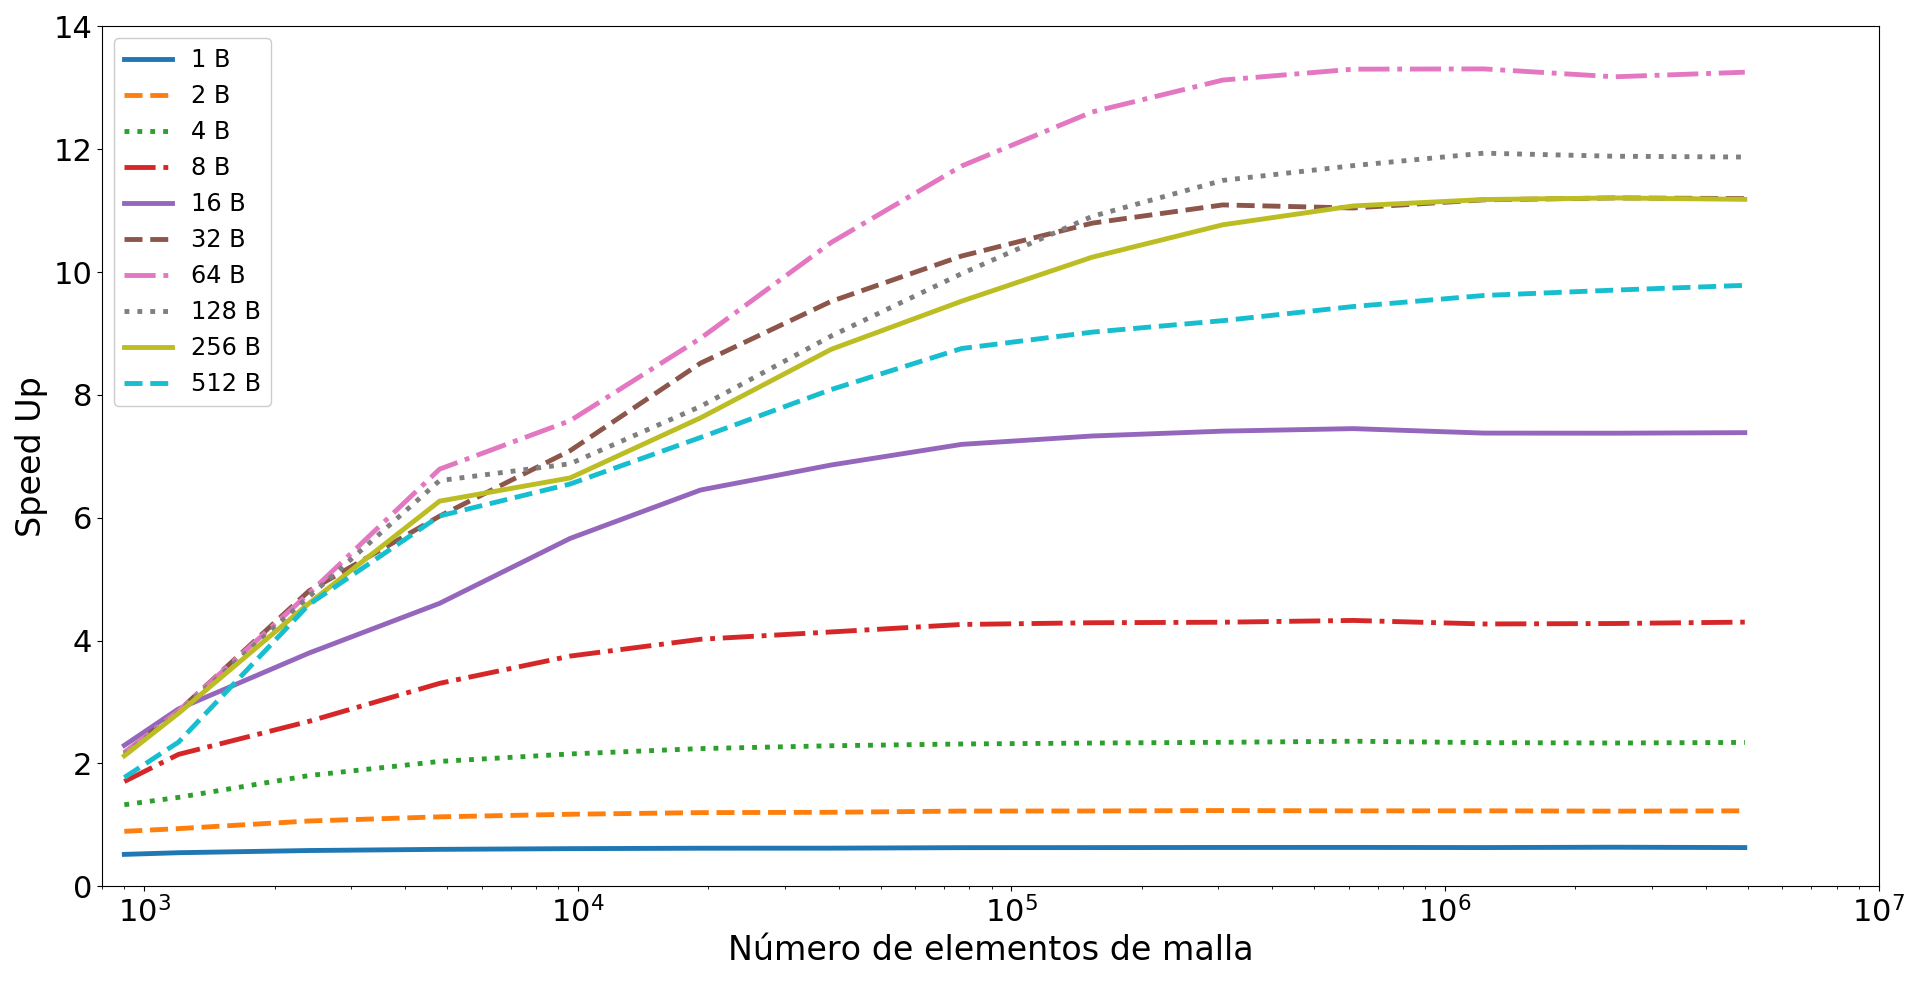
\includegraphics[width=\textwidth]{figs/cap4/s_760_VdW_simple_10}
	\caption{SU realizado para el problema de la Estratificación de un fluido Van dar Waals en simple precisión con una CPU Intel Core i7-3770 y GPU NVIDIA GeForce GTX 760.} 
	\label{fig:s_760_VdW_simple_10}	
\end{figure}

\begin{figure}[htbp]
	\centering
	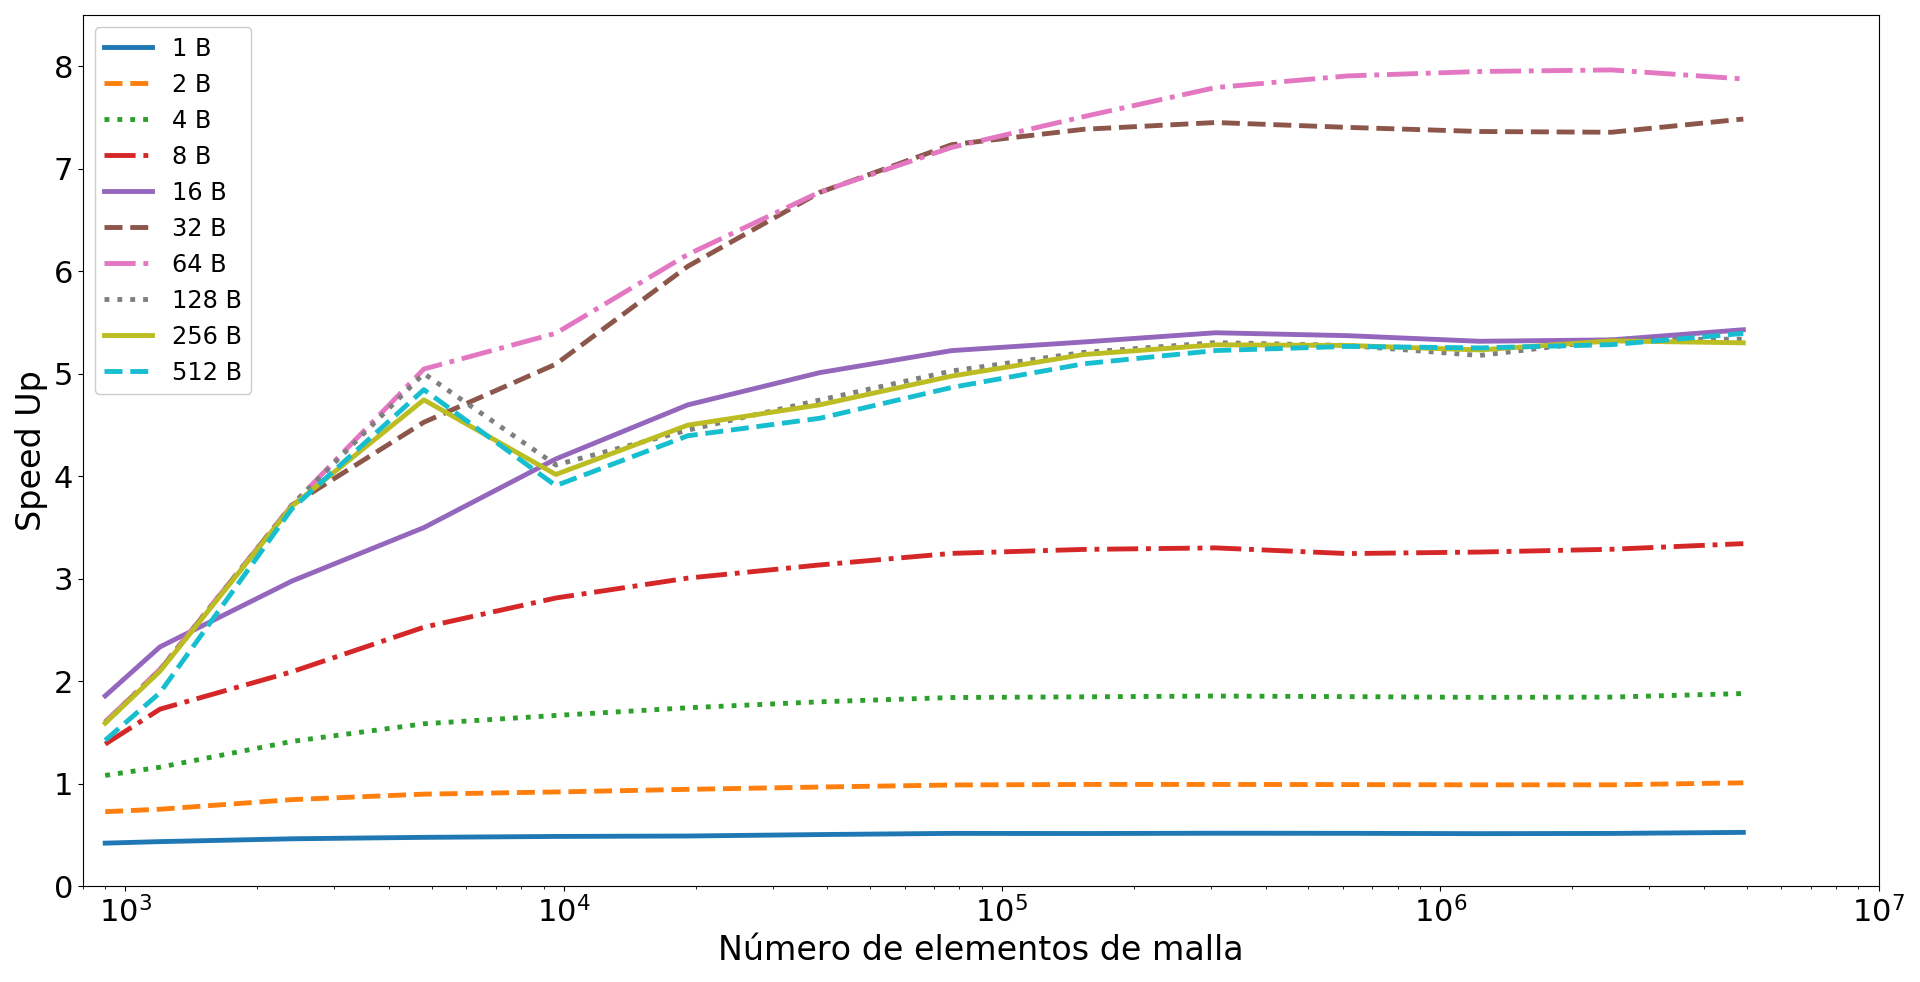
\includegraphics[width=\textwidth]{figs/cap4/s_760_VdW_double_10}
	\caption{SU realizado para el problema de la Estratificación de un fluido Van dar Waals en doble precisión con una CPU Intel Core i7-3770 y GPU NVIDIA GeForce GTX 760.} 
	\label{fig:s_760_VdW_double_10}	
\end{figure}

La Figura (\ref{fig:c_760_VdW_cuda_10}) muestra el ${SU}_p$ del código de \textsc{Cuda C} en la GPU NVIDIA GeForce GTX 760. Para un número de \textit{thread block} igual a 64, el tiempo de cálculo en doble precisión es 1,77 veces mayor que en simple precisión en el mayor número de elementos de malla calculado. Se reporta únicamente el resultado para esa cantidad de \textit{thread block}, debido a que los resultados anteriores indican que es el que tiene un mayor SU.

\begin{figure}[h!]
	\centering
	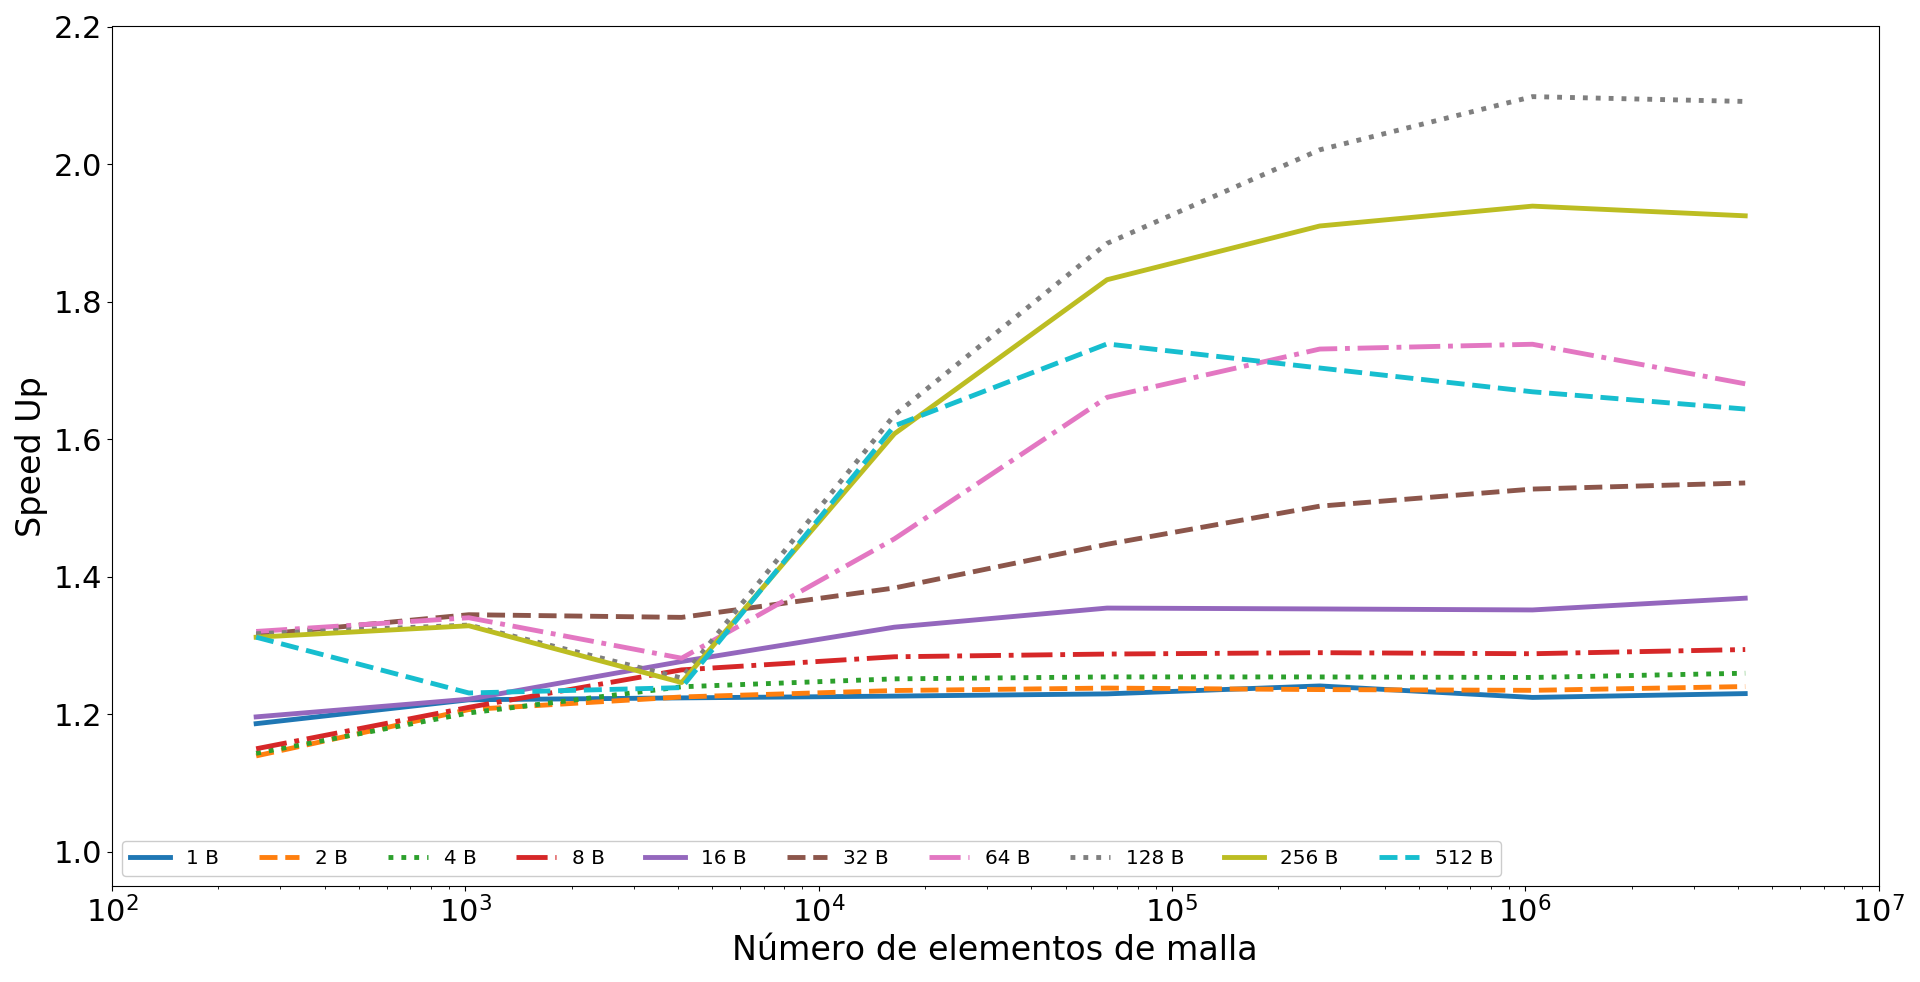
\includegraphics[width=\textwidth]{figs/cap4/c_760_MxC_cuda_10}
	\caption{$SU_p$ realizado para el problema de la Estratificación de un fluido Van der Waals en en el código de \textsc{Cuda C} con la GPU NVIDIA GeForce GTX 760.} 
	\label{fig:c_760_VdW_cuda_10}	
\end{figure}

\newpage

\subsubsection{NVIDIA GeForce GTX 970}

Los tamaños de grilla que se utilizaron para realizar las pruebas de tiempo de esta placa, tienen el rango de grilla de 3x300 nodos hasta 1638400x300 nodos. La cantidad de \textit{thread blocks} que se utilizó fueron de 1 a 512.



\begin{figure}[h!]
	\centering
	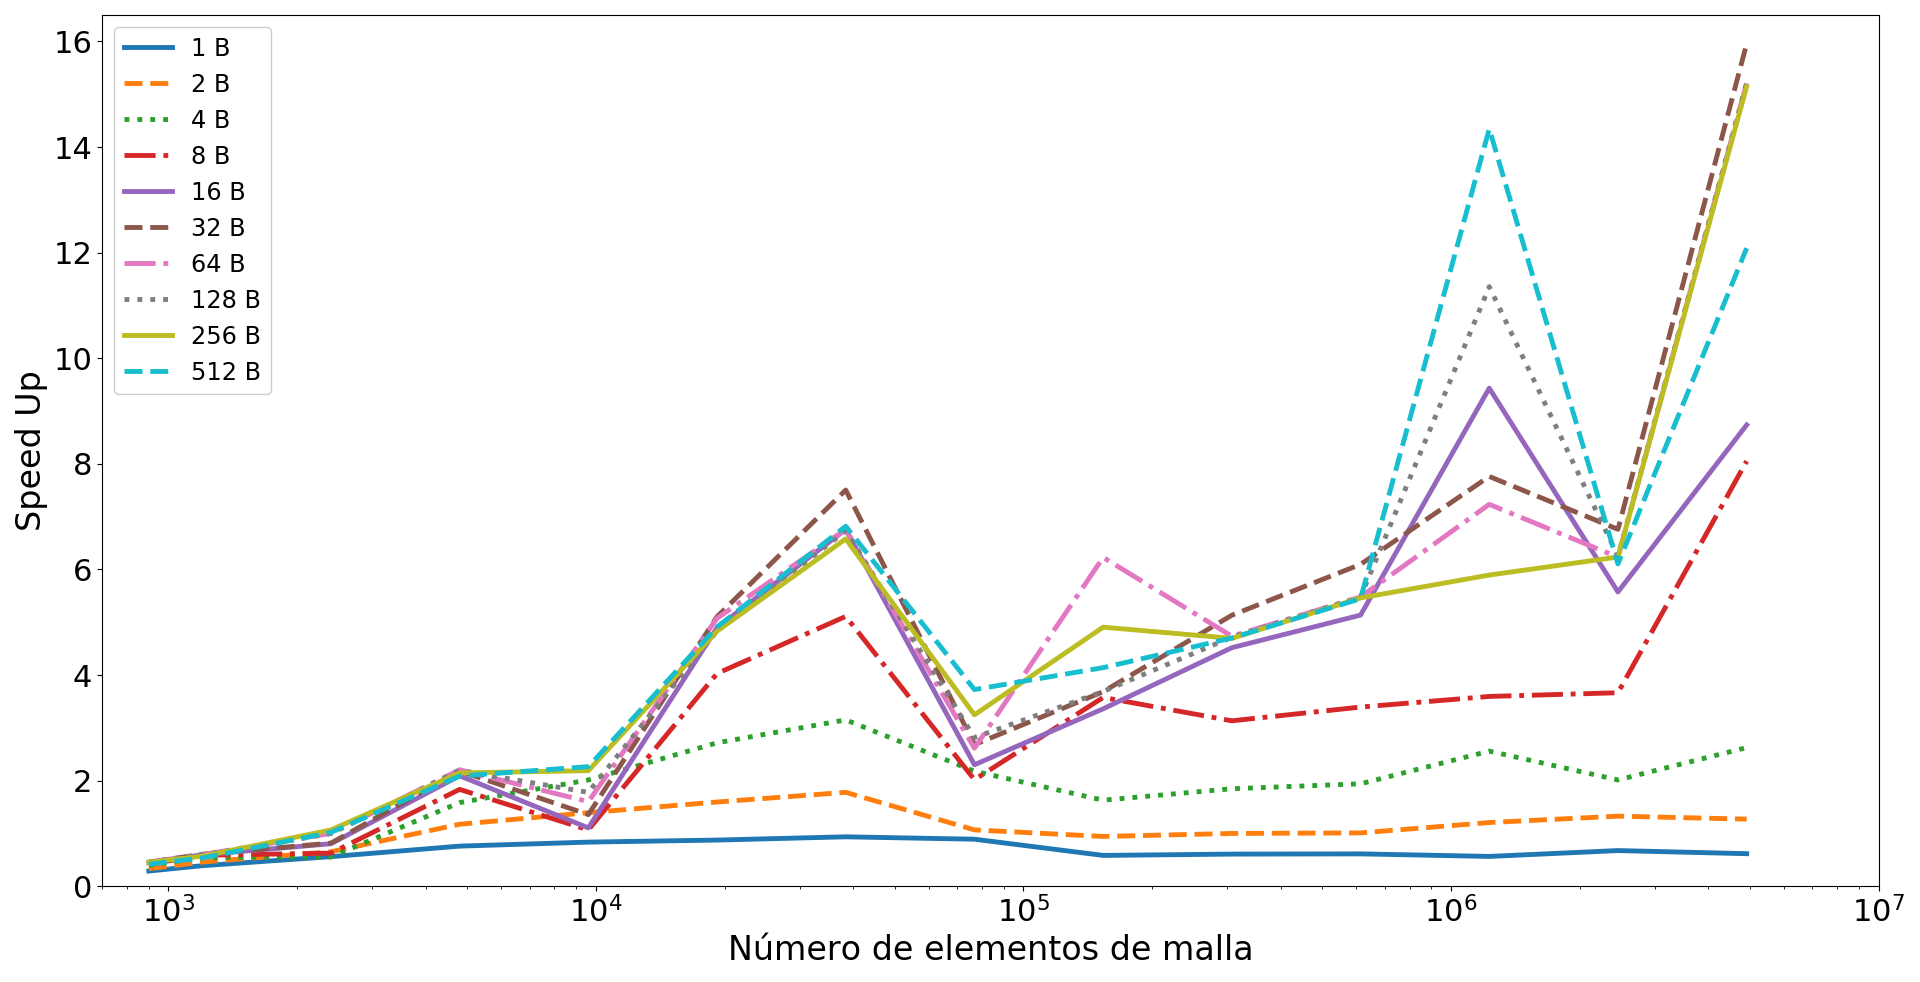
\includegraphics[width=\textwidth]{figs/cap4/s_970_VdW_simple_10}
	\caption{SU realizado para el problema de la Estratificación de un fluido Van dar Waals en simple precisión con una CPU Intel Core i7-4770 y GPU NVIDIA GeForce GTX 970.} 
	\label{fig:s_970_VdW_simple_10}	
\end{figure}

\begin{figure}[h!]
	\centering
	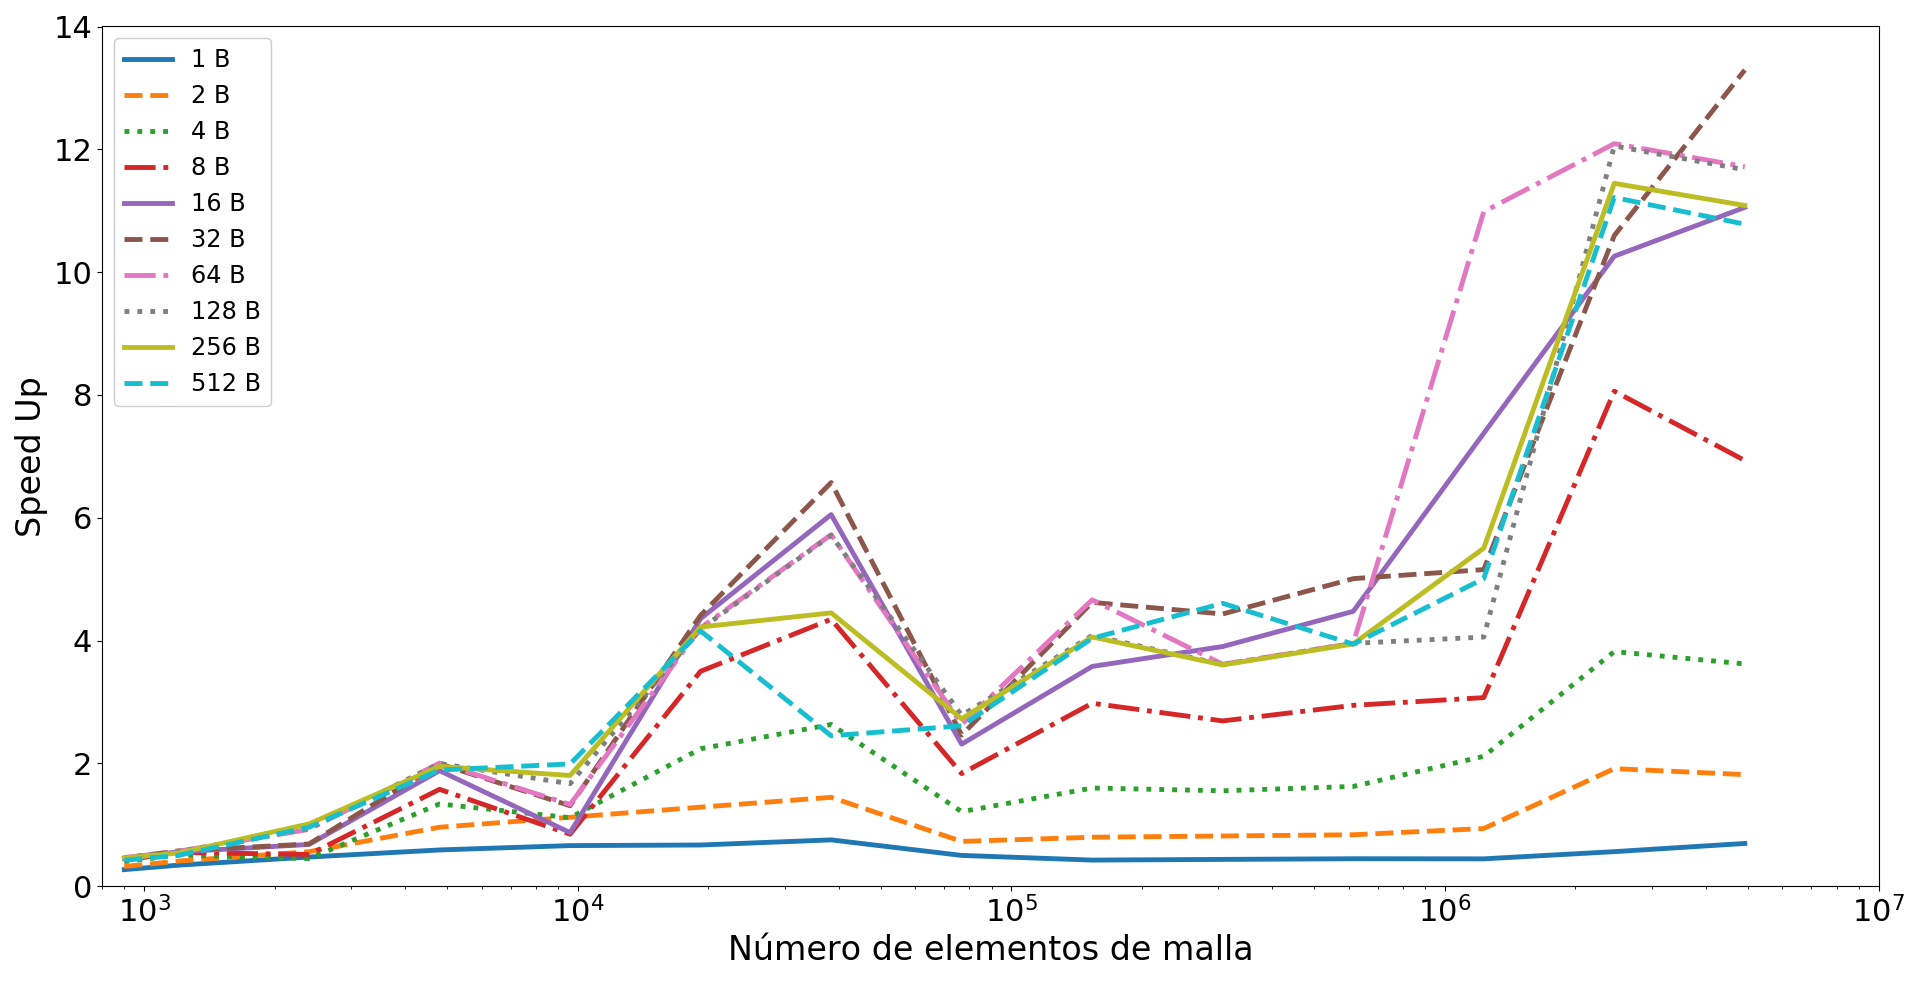
\includegraphics[width=\textwidth]{figs/cap4/s_970_VdW_double_10}
	\caption{SU realizado para el problema de la Estratificación de un fluido Van dar Waals en doble precisión con una CPU Intel Core i7-4770 y GPU NVIDIA GeForce GTX 970.} 
	\label{fig:s_970_VdW_double_10}	
\end{figure}

\newpage

Las Figuras (\ref{fig:s_970_VdW_simple_10}) y (\ref{fig:s_970_VdW_double_10}) muestran el \textit{SU} obtenido en simple precisión y doble precisión respectivamente. El mejor resultado en ambos casos se obtuvo para un número de \textit{thread block} igual a 32, donde la mejora fue de 15.95 y 13.29 en simple y doble precisión respectivamente, para el mayor número de elementos de malla.

La Figura (\ref{fig:c_970_VdW_cuda_10}) muestra el ${SU}_p$ del código de \textsc{Cuda C} en la GPU NVIDIA GeForce GTX 760. Para un número de \textit{thread block} igual a 32, el tiempo de cálculo en doble precisión es 1,25 veces mayor que en simple precisión en el mayor número de elementos de malla calculado. Se reporta únicamente el resultado para esa cantidad de \textit{thread block}, debido a que los resultados de las Figuras (\ref{fig:s_760_VdW_simple_10}) y (\ref{fig:s_760_VdW_double_10}) indican que es el que tiene un mayor SU.


\begin{figure}[h!]
	\centering
	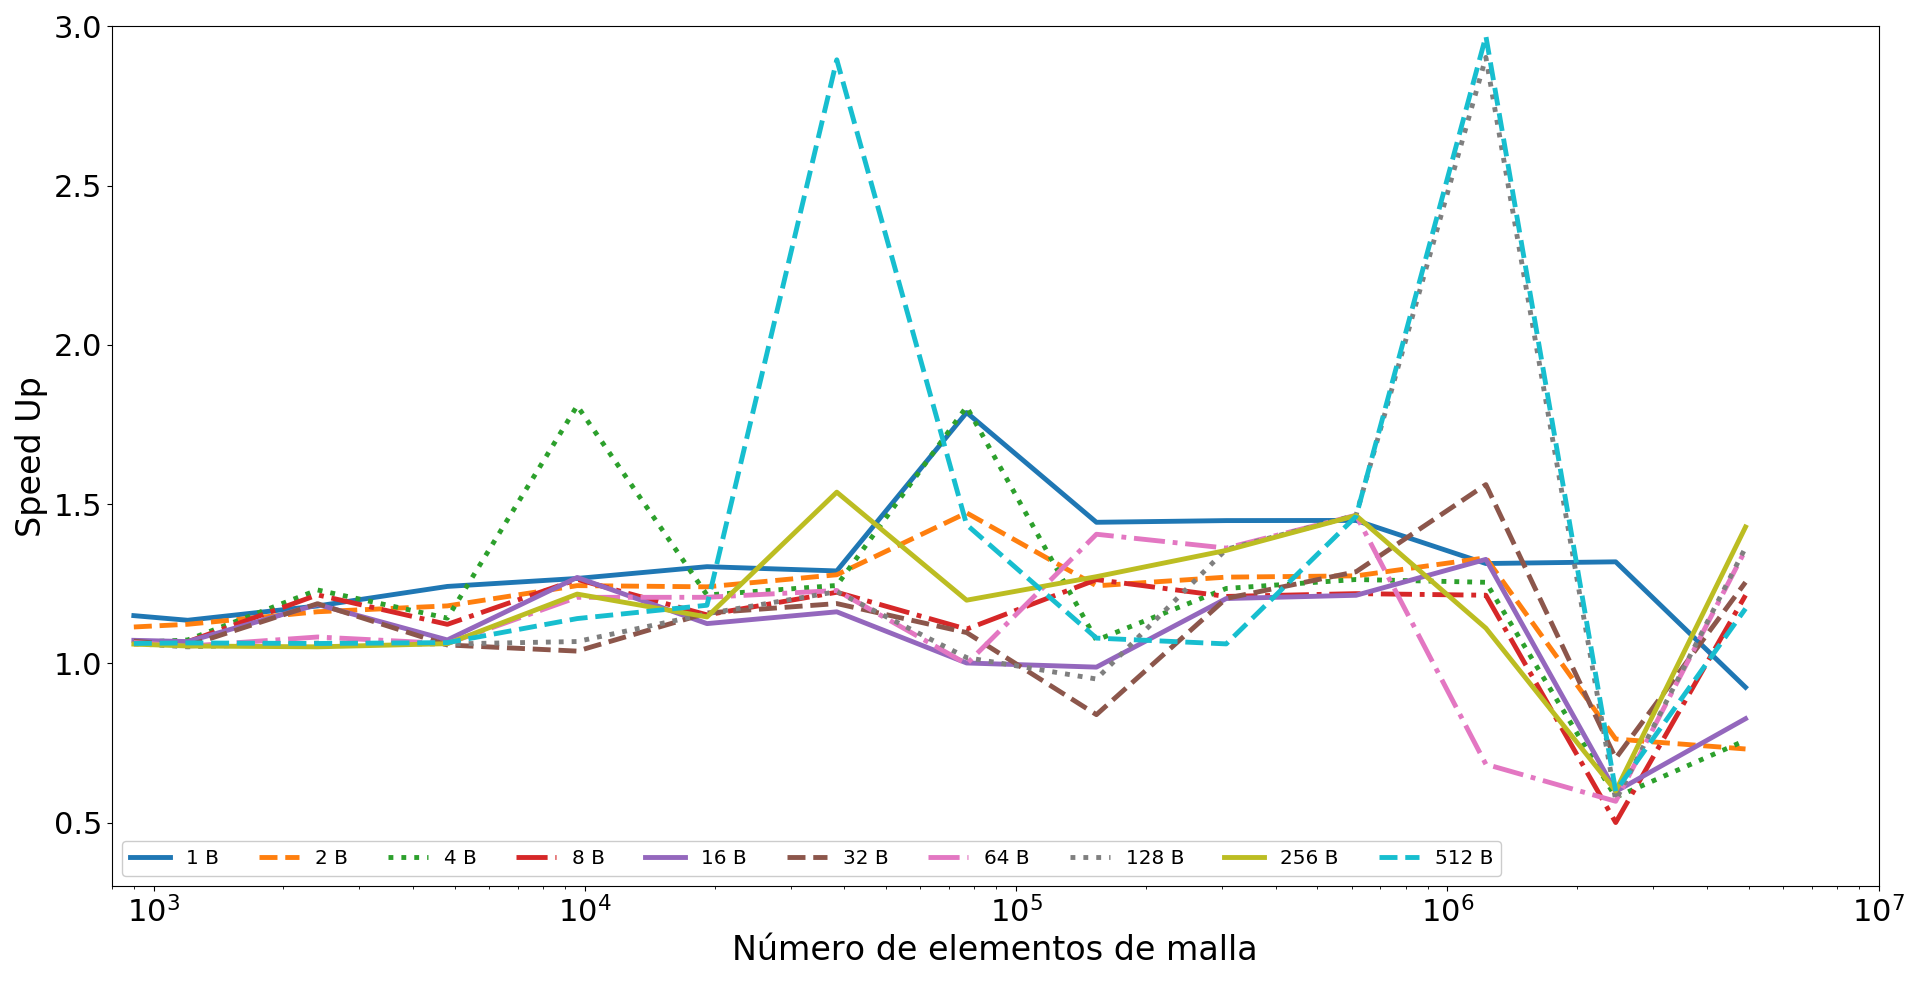
\includegraphics[width=\textwidth]{figs/cap4/c_970_VdW_cuda_10}
	\caption{$SU_p$ realizado para el problema de la Estratificación de un fluido Van der Waals en en el código de \textsc{Cuda C} con la GPU NVIDIA GeForce GTX 970.} 
	\label{fig:c_970_VdW_cuda_10}	
\end{figure}

\section{Resultados con \textsc{Python}}

La realización de los códigos numéricos mediante \textsc{C} y \textsc{Cuda C} tenian como primera finalidad conocer cuál es la ganancia en tiempo de cálculo realizando la implementación en GPU, y su otra finalidad era  realizar un código en \textsc{Cuda C}, para luego compilarlo en formato \textsc{ptx} y ser utilizado en \textsc{Python} por medio del módulo \textsc{PyCuda} del mismo.

Por falta de tiempo, no se pudo hacer un código en \textsc{Python} que resuelva los problemas mecionados en el presente capítulo. Lo que se realizó fue un \textit{SU} 
de uno de las \textit{kernel} del código, el cual resuelve la Ec.(\ref{eq:rho_py}):

\begin{equation}
\rho = \sum_{\alpha} f_{\alpha}
\label{eq:rho_py}
\end{equation}

Para éste análisis se inicializó a $f$ con valores aleatorios, haciendo una repetición de la ejecución de la función 100000 veces para realizar la toma de tiempo. Se varió el tamaño de la grilla, de manera que ésta siempre fuese cuadrada, respetando un número de nodos de potencia de 2 en los lados del cuadrado. La cantidad de \textit{thread blocks} que se utilizó para realizar la comparación en el código fue de potencia de 2. El tamaño de la grilla varió de 16x16 hasta 4096x4906 y la cantidad de \textit{thread blocks} utilizado es de 1 a 512.

\newpage

Al  realizar la implementación de un \textit{kernel} de \textsc{Cuda C} en \textsc{Python}, se espera que el tiempo de cálculo en \textsc{Python} sea más lento que en \textsc{Cuda C}, debido a que el primer lenguaje es interpretado. Debido a lo mencionado es que se define el índice \textit{Speed Down} (SD), que resulta ser una medida de cuánto es la demora de un código respecto a otro y se calcula de la siguiente forma :

\begin{align}
	SD = \frac{t_{\>PyCuda}}{t_{\>Cuda \> C}} 
\end{align} 


\title{\textbf{NVIDIA GeForce GTX 760}}

La Figura (\ref{fig:s_cuda_760_test_simple_10}) muestra el SU para la GPU NVIDIA GeForce GTX 760, en donde la mayor ganancia se obtuvo que para 64 \textit{thread blocks}, siendo de 3.198. La Figura (\ref{fig:s_py_760_test_simple_10}) muestra el $SD$, en donde sobtuvo que para 128 y 512  \textit{thread blocks} se obtuvo el menor incremento de tiempos de cálculo, siendo de 1.144. 

\begin{figure}[h!]
	\centering
	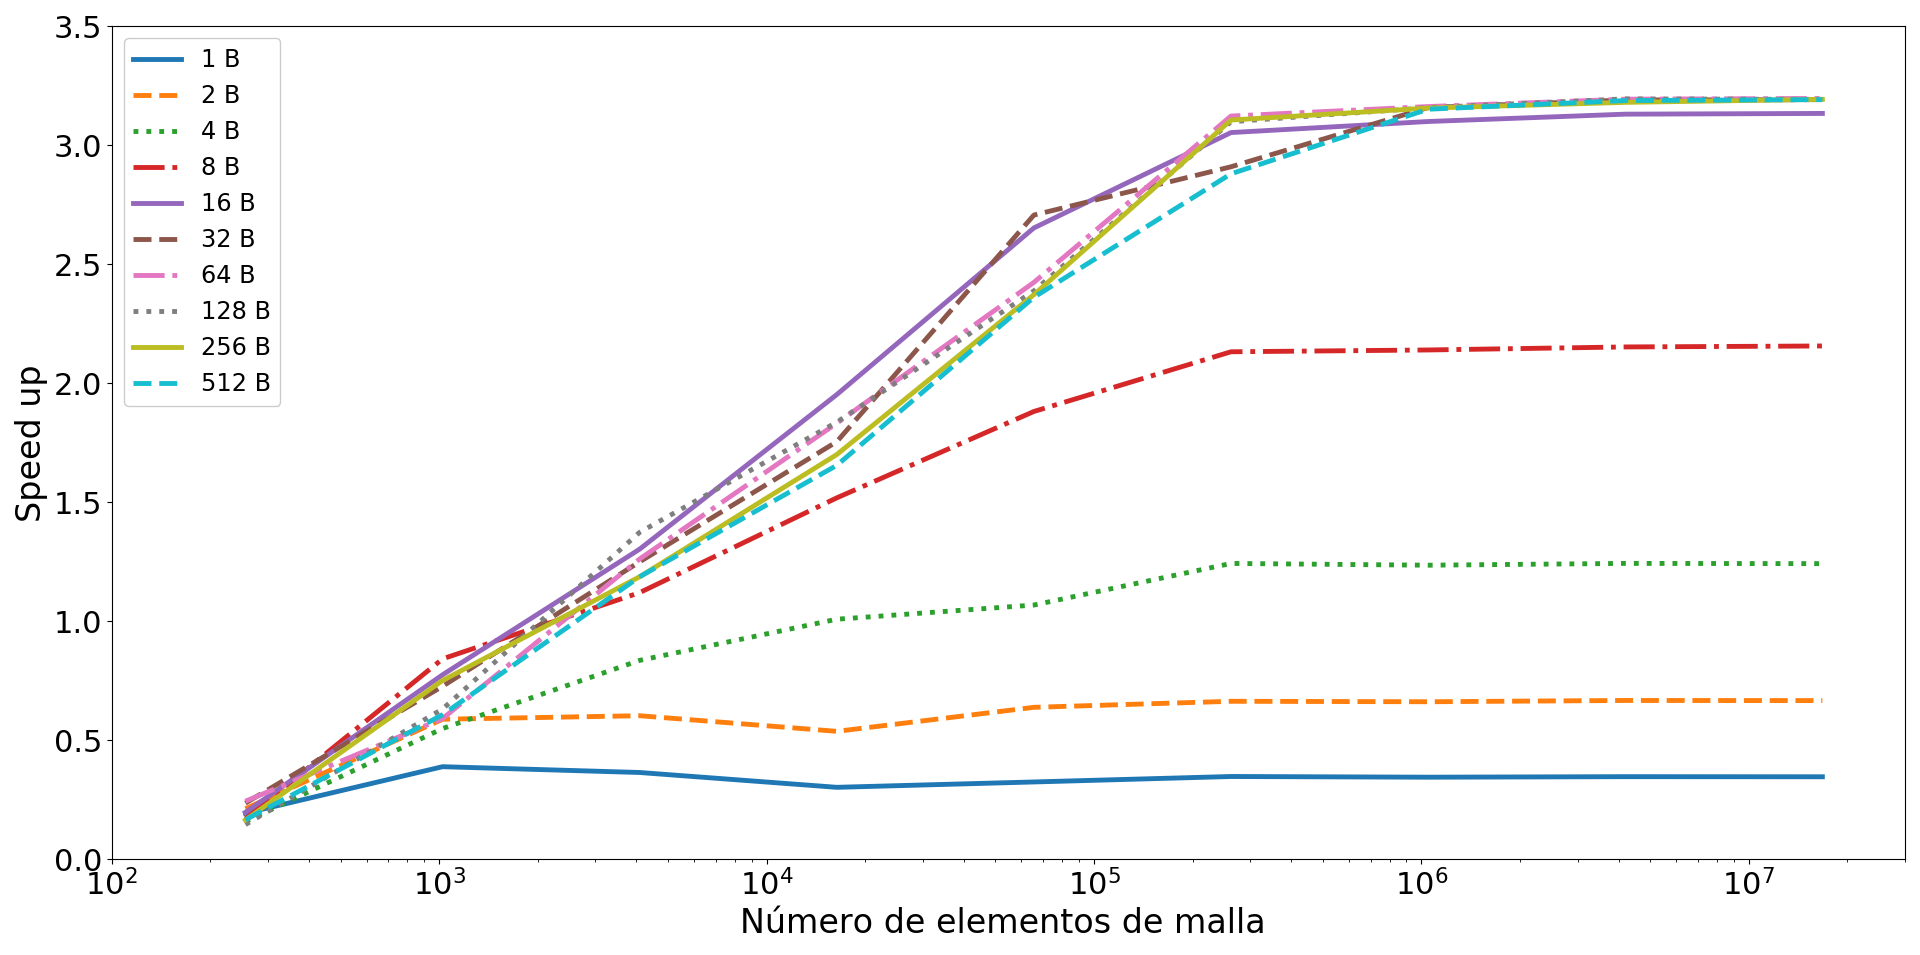
\includegraphics[width=\textwidth]{figs/cap4/s_cuda_760_test_simple_10}
	\caption{SU entre \textsc{C} y \textsc{Cuda C} para la función de obtensión de la densidad con la GPU NVIDIA GeForce GTX 760 en simple precisión.} 
	\label{fig:s_cuda_760_test_simple_10}	
\end{figure}

%\begin{figure}[h!]
%	\centering
%	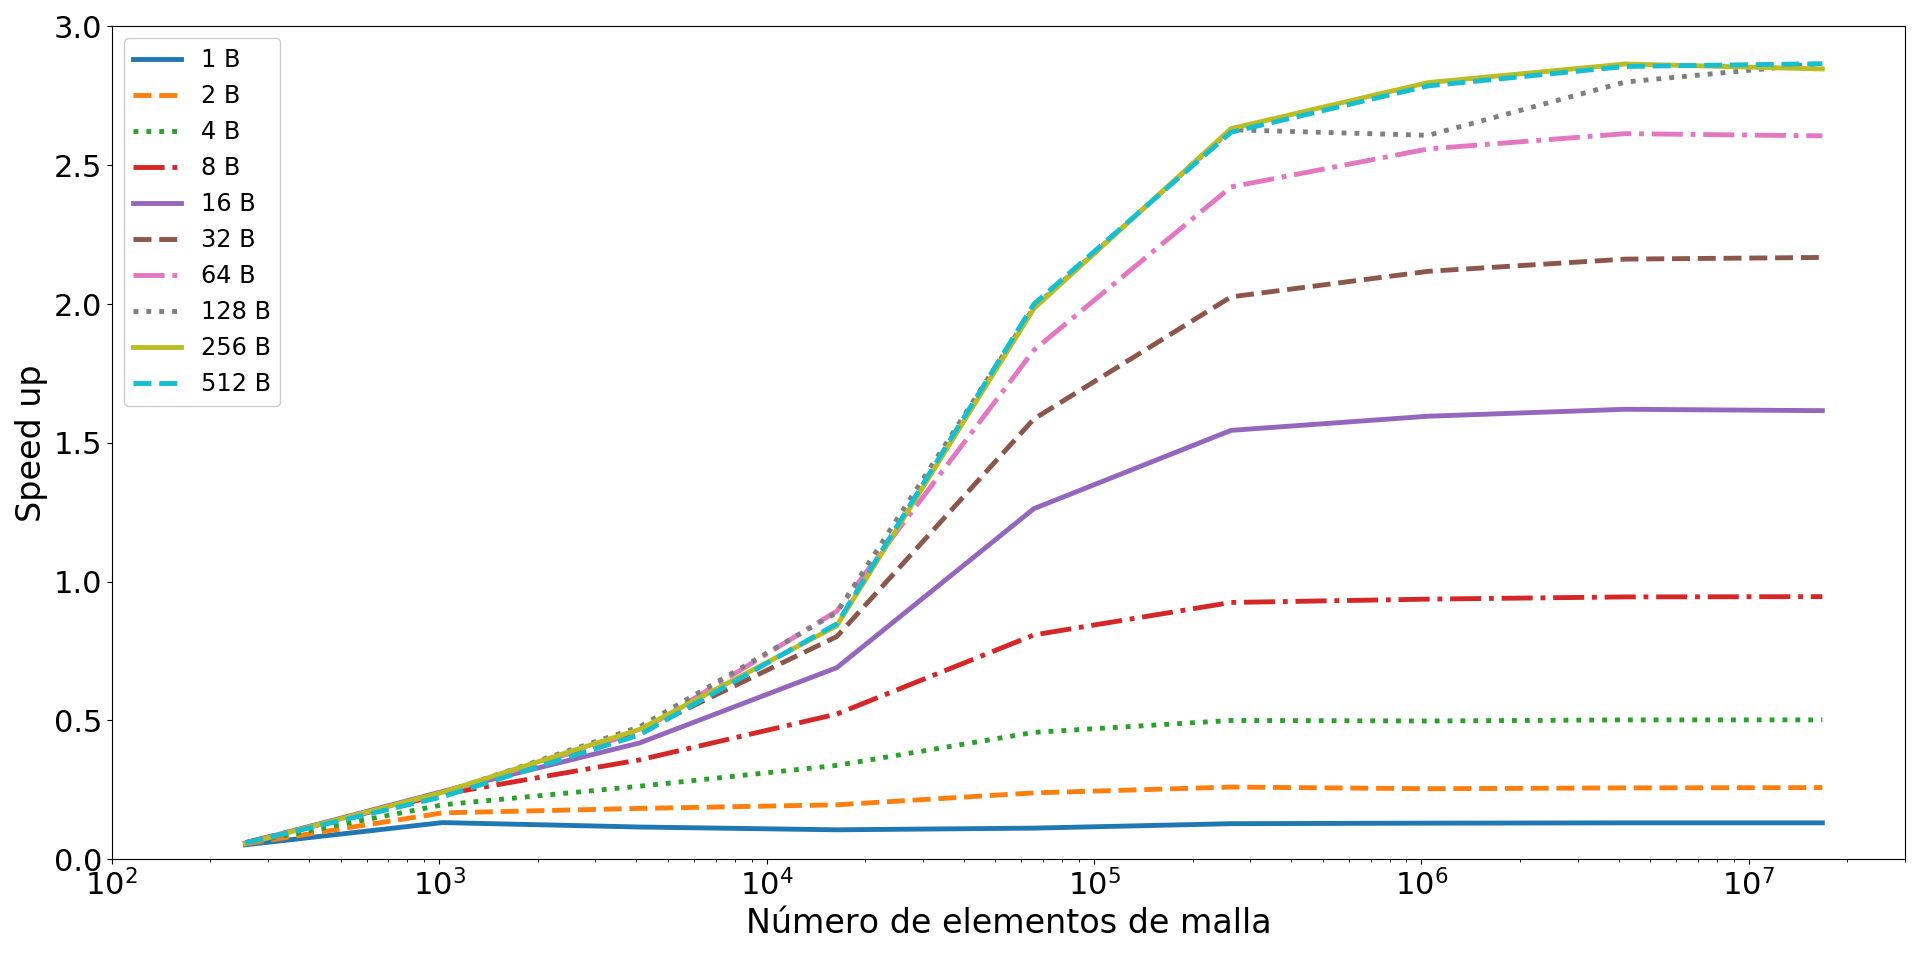
\includegraphics[width=\textwidth]{figs/cap4/s_py_c_760_test_simple_10}
%	\caption{Speed Up realizado entre PyCUDA y C para la función de obtensión de la densidad con la GPU NVIDIA GeForce GTX 760 en simple precisión.} 
%	\label{fig:s_py_c_760_test_simple_10}	
%\end{figure}


\begin{figure}[h!]
	\centering
	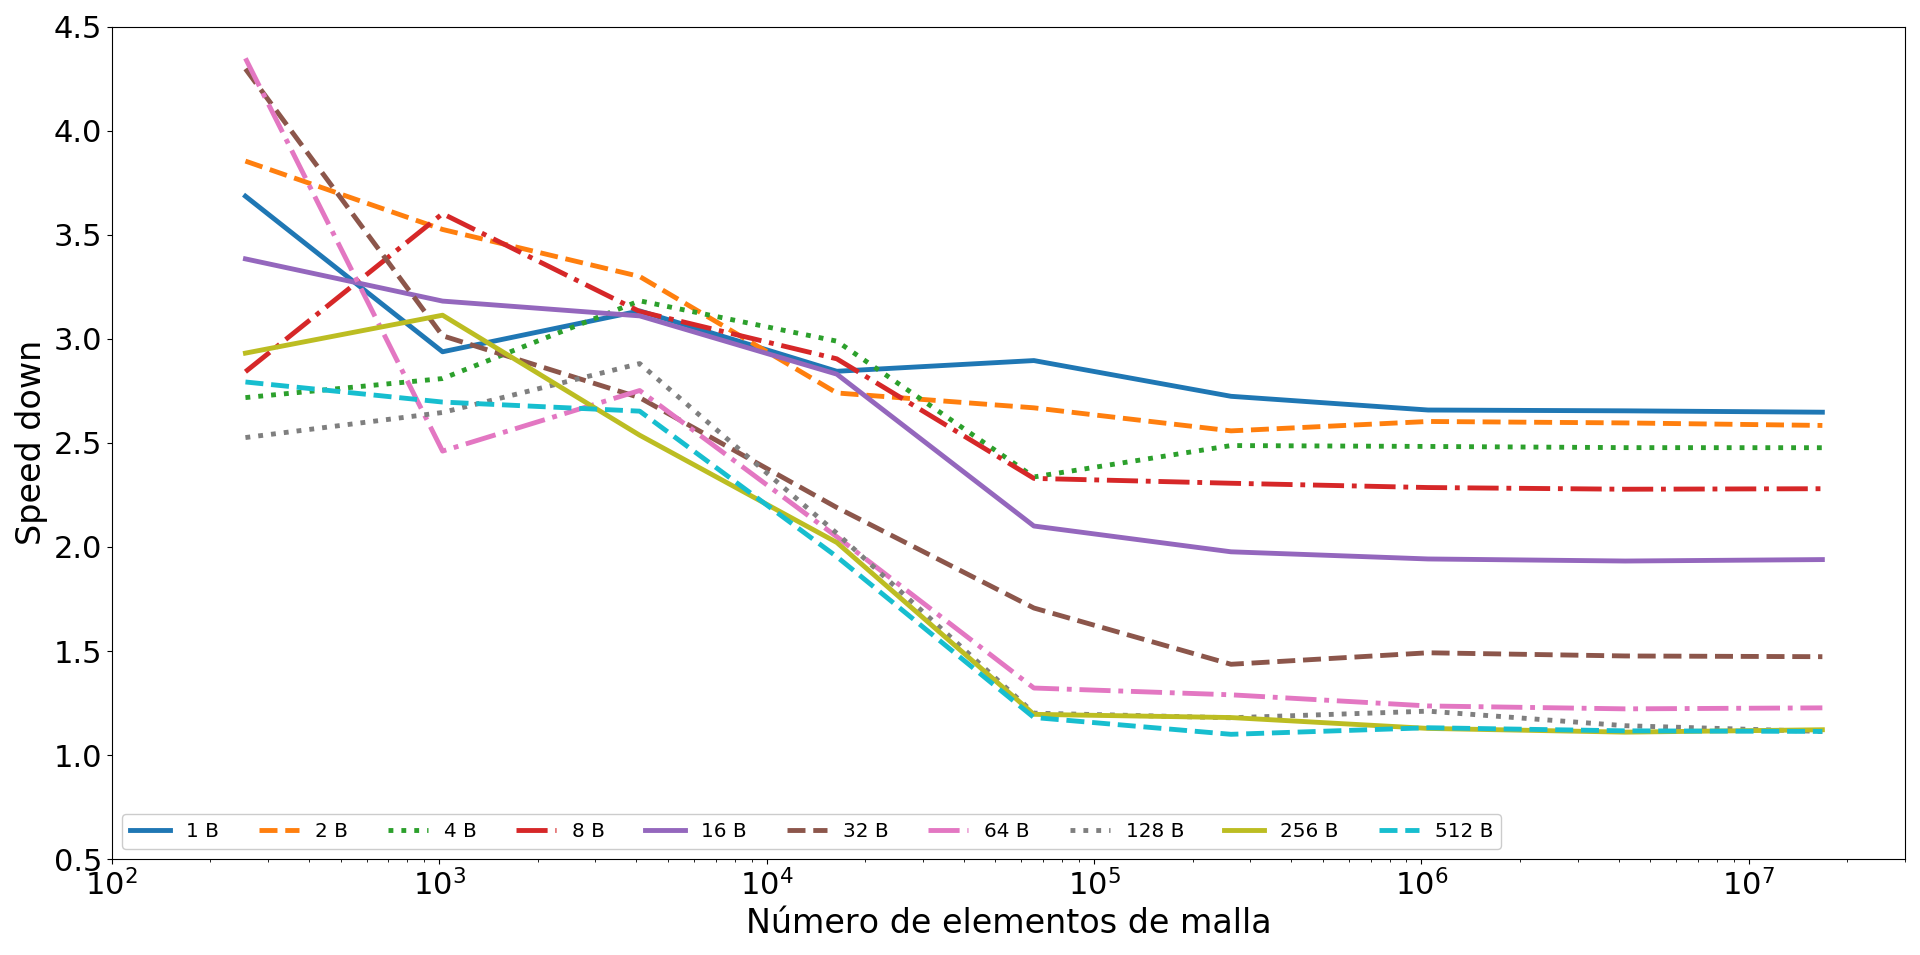
\includegraphics[width=\textwidth]{figs/cap4/s_py_760_test_simple_10}
	\caption{SD realizado entre PyCUDA y CUDA para la función de obtensión de la densidad con la GPU NVIDIA GeForce GTX 760 en simple precisión.} 
	\label{fig:s_py_760_test_simple_10}	
\end{figure}



%
\title{\textbf{NVIDIA GeForce GTX 970}}

La Figura (\ref{fig:s_cuda_970_test_simple_10}) muestra la ganancia obtenida en el código de \textsc{Cuda C} sobre \textsc{C}. Para 64 \textit{thread blocks} se obtuvo la mayor ganancia, siendo de 4.815. La Figura (\ref{fig:s_py_c_970_test_simple_10}) muestra la ganancia obtenida en el código de \textsc{PyCuda} sobre \textsc{C}. Para 256 \textit{thread blocks} se obtuvo la mayor ganancia, siendo de 4.242. La Figura (\ref{fig:s_py_970_test_simple_10}) muestra cuanto más se demora el código de \textsc{PyCuda} con respecto al de \textsc{Cuda C}. Para 512  \textit{thread blocks} se obtuvo el menor incremento de tiempos de cálculo, siendo de 1.087; y para 256 \textit{thread blocks} es de 1.104 veces.

\begin{figure}[htbp]
	\centering
	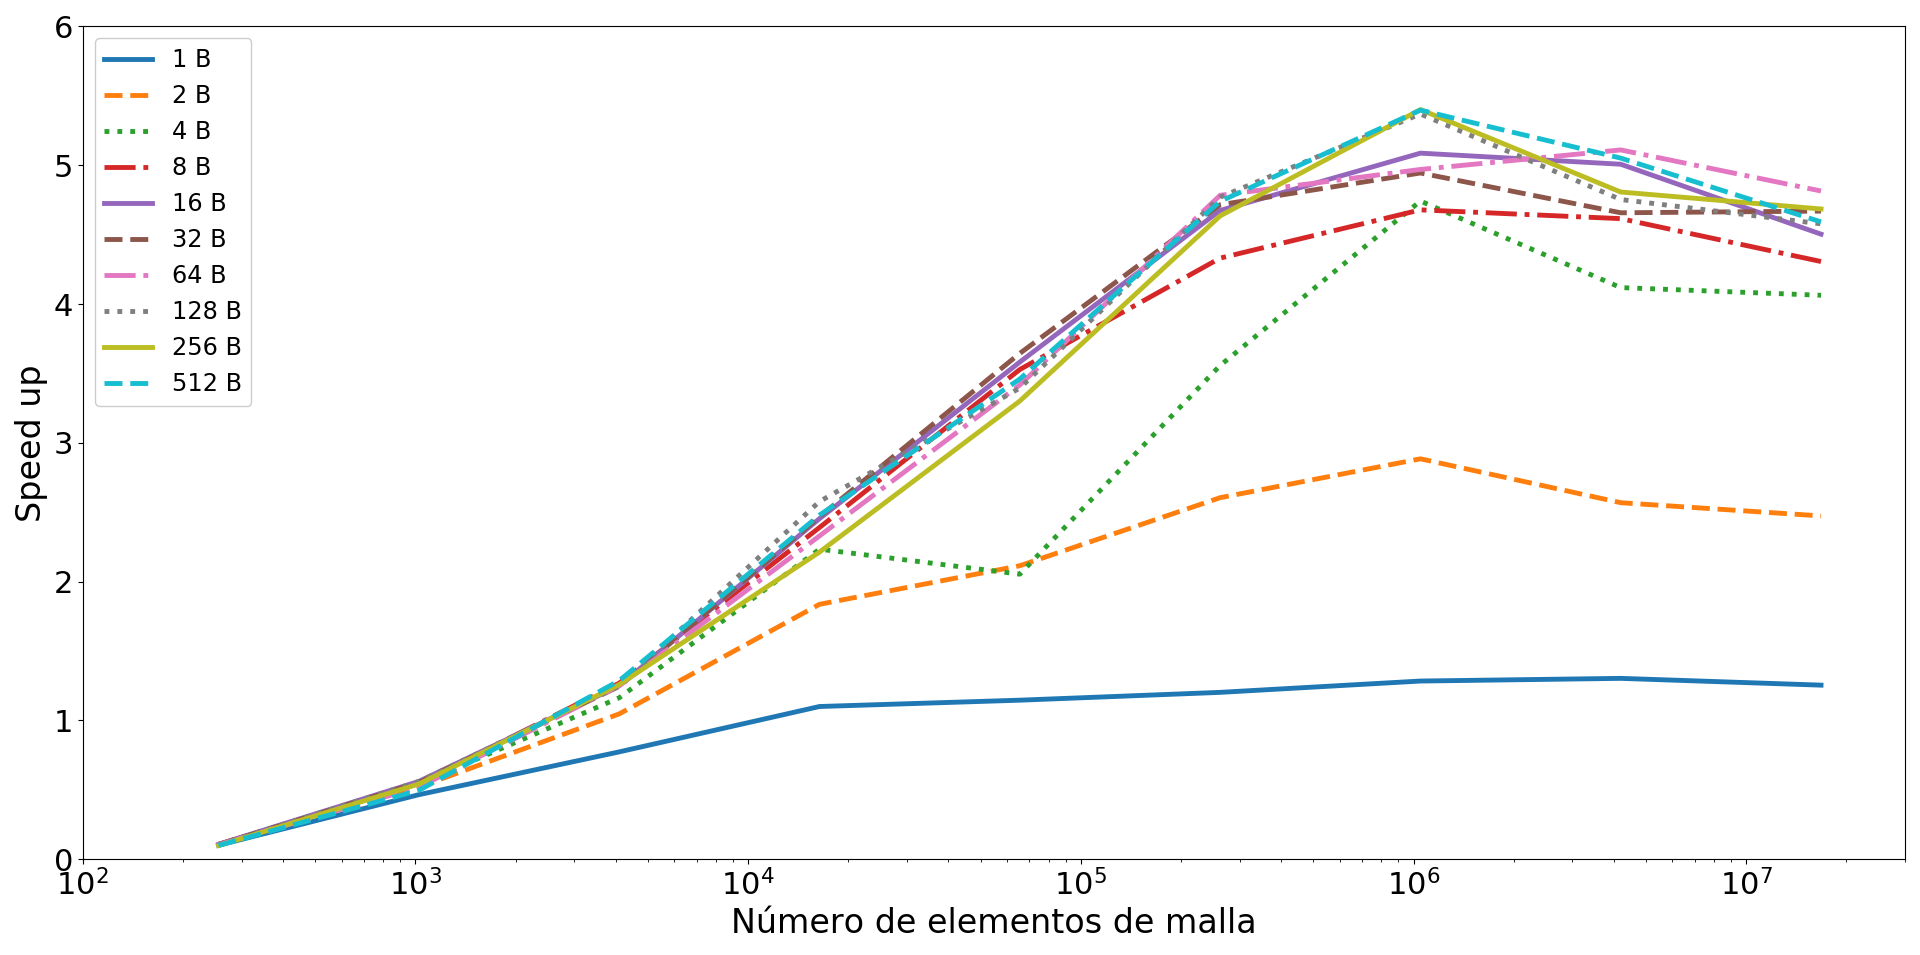
\includegraphics[width=\textwidth]{figs/cap4/s_cuda_970_test_simple_10}
	\caption{SU realizado entre \textsc{C} y \textsc{Cuda C} para la función de obtensión de la densidad con la GPU NVIDIA GeForce GTX 970 en simple precisión.} 
	\label{fig:s_cuda_970_test_simple_10}	
\end{figure}

%\begin{figure}[htbp]
%	\centering
%	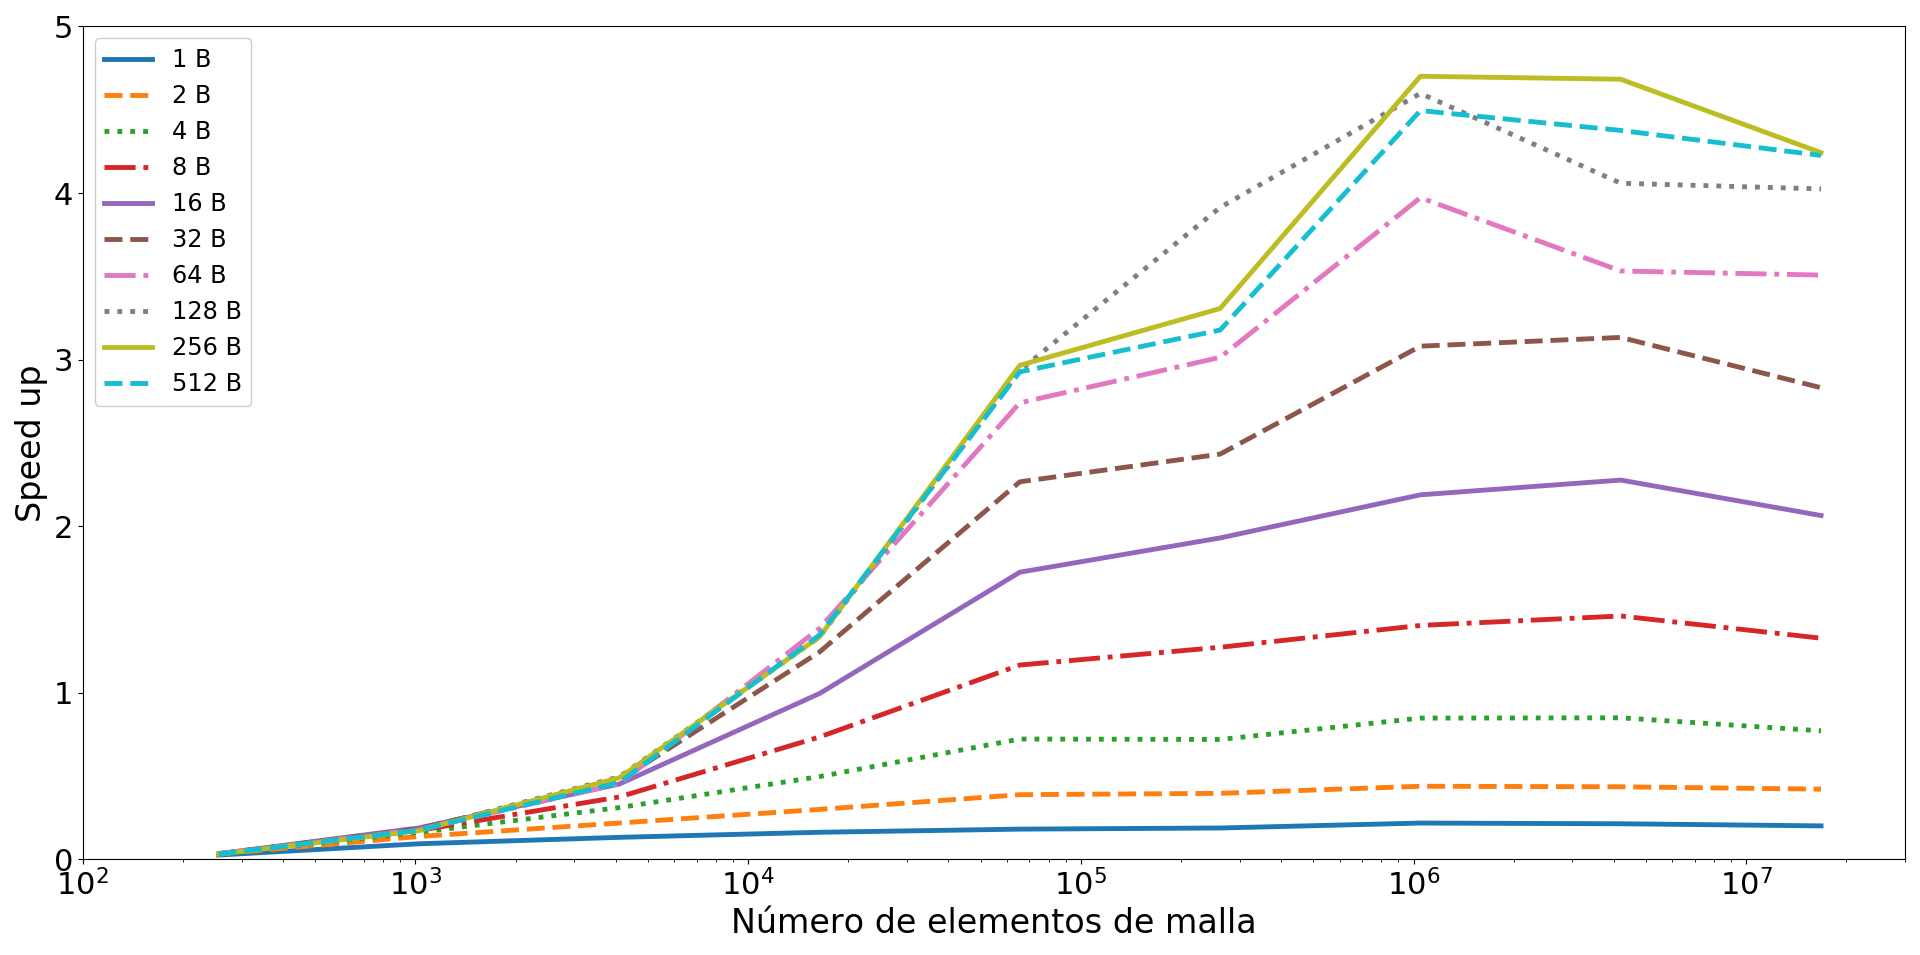
\includegraphics[width=\textwidth]{figs/cap4/s_py_c_970_test_simple_10}
%	\caption{Speed Up realizado entre PyCUDA y C para la función de obtensión de la densidad con la GPU NVIDIA GeForce GTX 970 en simple precisión.} 
%	\label{fig:s_py_c_970_test_simple_10}	
%\end{figure}

\begin{figure}[htbp]
	\centering
	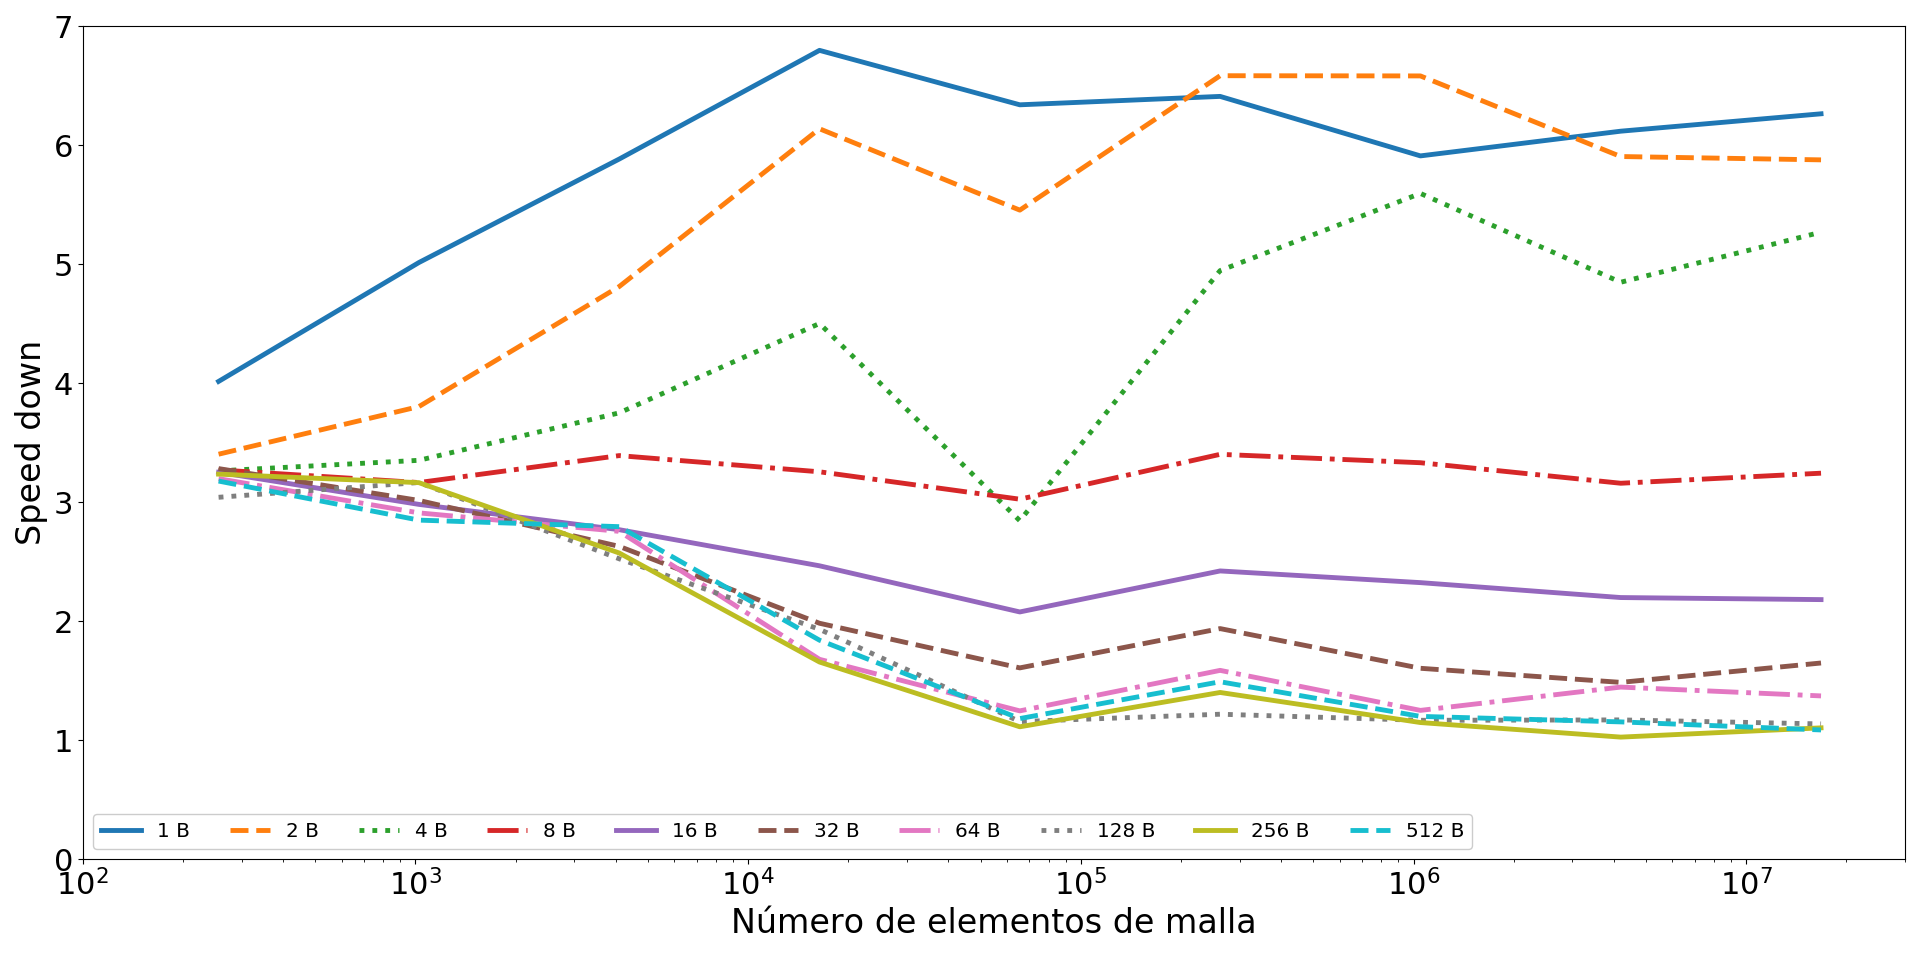
\includegraphics[width=\textwidth]{figs/cap4/s_py_970_test_simple_10}
	\caption{SU realizado entre \textsc{PyCuda} y \textsc{Cuda C} para la función de obtensión de la densidad con la GPU NVIDIA GeForce GTX 970 en simple precisión.} 
	\label{fig:s_py_970_test_simple_10}	
\end{figure}

\section{Análisis}

Según los resultados obtenidos, se espera que utilizando la cantidad de \textit{thread blocks} que maximicen la ganancia en un código de \textsc{Python} sobre el código de \textsc{C}, el primero posea un incremento de un  15 \%  u 10 \% en comparación con el código de \textsc{Cuda C}, si es que se utiliza una GPU NVIDIA GeForce GTX 760/970 respectivamente.

Por lo que no se pierde mucha eficiencia programando en el lenguaje de \textsc{Python}.

\newpage
\section{Generación de burbujas sobre una superficie horizontal calefaccionada}

Mediante éste problema se quiere reproducir el fenómeno de ebullición nucleada. El trabajo en los dos problemas anteriores constituyen pasos para validar por partes el código. Ésto se debe a que el problema de la Construcción de Maxwell utiliza solamente una ecuación pseudopotencial, mientras que el problema de la estratificación de un fluido VdW utiliza las dos operaciones pseudopotenciales planteadas.

La diferencia del problema de la estratificación de VdW con el de la generación de burbujas, radica en que el primero es unidimensional, el segundo es bidimensional. A su vez, la aplicación del código cambia únicamente en realizar una función que imponga como condición de contorno un área de la superficie calefaccionada.

El valor de $\mathbf{M}$ utilizado es el mismo que los probelmas anteriores, el resto de los parámetros se encuentran en el Apéndice (\ref{parametros_bub}).

Los resultados que se obtuvieron se encuentra en las Figura (\ref{fig:secuencia_burbujas}), donde los tiempos de vuelo mostrados son de 5000, 10000, 20000, 25000, 30000, 35000, 40000, 45000 y 5000 pasos. El tamaño de grilla utilizado fue de L = 300 y H = 500, si se toma como esquema el mostrado en la Figura(\ref{fig:esquema_VdW}). La superficie calefaccionada se encuentra en el centro del lado L y posee un tamaño de 24 elementos de malla, siendo la temperatura de calefacción $T_{heat} = T_c$. El resto de la superficie se encuentra a $T = 0.8 T_c$ y la parte superior de la cavidad está a $T = 0.99 T_c$. La separación inicial de las dos fases se encuentra en $y = 350$, donde $\rho = 0.1610588 \> sii \> y \in [0,350]$ y $\rho = 0.0199722 \>\> y \in (350,500]$.

\begin{figure}[h!]
	\centering
	\begin{subfigure}{0.25\textwidth}
		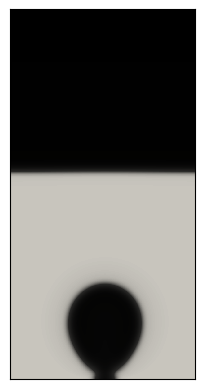
\includegraphics[width=\linewidth]{figs/cap4/bubble_5}
		\caption{t = 5000}
		\label{fig:1}
	\end{subfigure}\hfil 
	\begin{subfigure}{0.25\textwidth}
		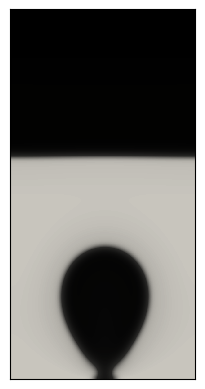
\includegraphics[width=\linewidth]{figs/cap4/bubble_10}
		\caption{t = 10000}
		\label{fig:2}
	\end{subfigure}\hfil 
	\begin{subfigure}{0.25\textwidth}
		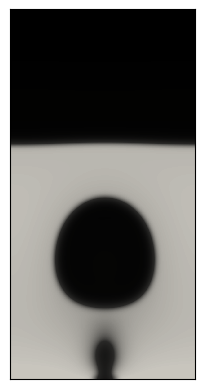
\includegraphics[width=\linewidth]{figs/cap4/bubble_20}
		\caption{t = 20000}
		\label{fig:3}
	\end{subfigure}
	
	\medskip
	\begin{subfigure}{0.25\textwidth}
		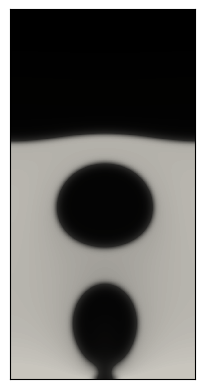
\includegraphics[width=\linewidth]{figs/cap4/bubble_25}
		\caption{t = 25000}
		\label{fig:4}
	\end{subfigure}\hfil  
	\begin{subfigure}{0.25\textwidth}
		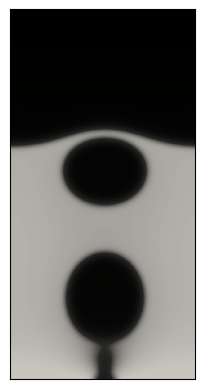
\includegraphics[width=\linewidth]{figs/cap4/bubble_30}
		\caption{t = 30000}
		\label{fig:5}
	\end{subfigure}\hfil 
	\begin{subfigure}{0.25\textwidth}
		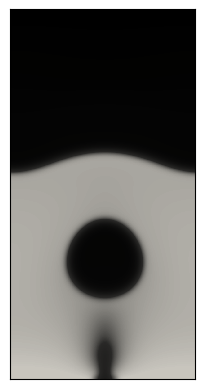
\includegraphics[width=\linewidth]{figs/cap4/bubble_35}
		\caption{t = 35000}
		\label{fig:6}
	\end{subfigure}
	
	\medskip
	\begin{subfigure}{0.25\textwidth}
		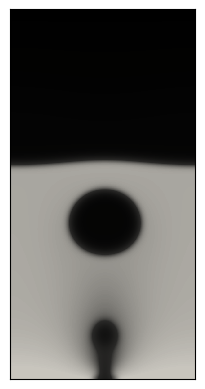
\includegraphics[width=\linewidth]{figs/cap4/bubble_40}
		\caption{t = 40000}
		\label{fig:7}
	\end{subfigure}\hfil
	\begin{subfigure}{0.25\textwidth}
		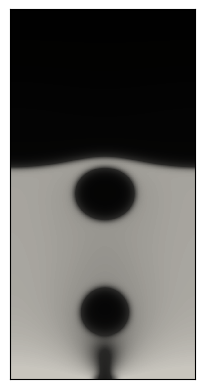
\includegraphics[width=\linewidth]{figs/cap4/bubble_45}
		\caption{t = 45000}
		\label{fig:8}
	\end{subfigure}\hfil 
	\begin{subfigure}{0.25\textwidth}
		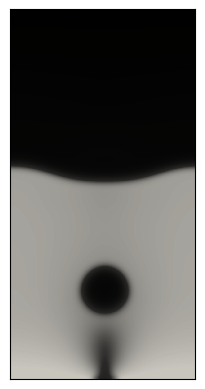
\includegraphics[width=\linewidth]{figs/cap4/bubble_50}
		\caption{t = 50000}
		\label{fig:9}
	\end{subfigure}
	\caption{Creación y desarrollo de una burbuja a partir de una superficie horizontal calefaccionada.}
	\label{fig:secuencia_burbujas}
\end{figure}



\newpage






%%% Local Variables: 
%%% mode: latex
%%% TeX-master: "template"
%%% End: 
